\documentclass[12pt,oneside]{article}
\usepackage[]{mathpazo}
\usepackage{amssymb,amsmath}
\usepackage{ifxetex,ifluatex}
\usepackage{fixltx2e} % provides \textsubscript
\ifnum 0\ifxetex 1\fi\ifluatex 1\fi=0 % if pdftex
  \usepackage[T1]{fontenc}
  \usepackage[utf8]{inputenc}
\else % if luatex or xelatex
  \ifxetex
    \usepackage{mathspec}
  \else
    \usepackage{fontspec}
  \fi
  \defaultfontfeatures{Ligatures=TeX,Scale=MatchLowercase}
\fi
% use upquote if available, for straight quotes in verbatim environments
\IfFileExists{upquote.sty}{\usepackage{upquote}}{}
% use microtype if available
\IfFileExists{microtype.sty}{%
\usepackage{microtype}
\UseMicrotypeSet[protrusion]{basicmath} % disable protrusion for tt fonts
}{}
\usepackage[margin=1in]{geometry}
\usepackage{hyperref}
\PassOptionsToPackage{usenames,dvipsnames}{color} % color is loaded by hyperref
\hypersetup{unicode=true,
            pdftitle={Application of Bayesian networks to mapping Flood-based Farming Systems.},
            pdfauthor={Issoufou Liman1,2,; Cory Whitney1,3; James Kungu2; Eike Luedeling1,3,4},
            colorlinks=true,
            linkcolor=blue,
            citecolor=red,
            urlcolor=blue,
            breaklinks=true}
\urlstyle{same}  % don't use monospace font for urls
\usepackage{longtable,booktabs}
\usepackage{graphicx,grffile}
\makeatletter
\def\maxwidth{\ifdim\Gin@nat@width>\linewidth\linewidth\else\Gin@nat@width\fi}
\def\maxheight{\ifdim\Gin@nat@height>\textheight\textheight\else\Gin@nat@height\fi}
\makeatother
% Scale images if necessary, so that they will not overflow the page
% margins by default, and it is still possible to overwrite the defaults
% using explicit options in \includegraphics[width, height, ...]{}
\setkeys{Gin}{width=\maxwidth,height=\maxheight,keepaspectratio}
\IfFileExists{parskip.sty}{%
\usepackage{parskip}
}{% else
\setlength{\parindent}{0pt}
\setlength{\parskip}{6pt plus 2pt minus 1pt}
}
\setlength{\emergencystretch}{3em}  % prevent overfull lines
\providecommand{\tightlist}{%
  \setlength{\itemsep}{0pt}\setlength{\parskip}{0pt}}
\setcounter{secnumdepth}{5}

%%% Use protect on footnotes to avoid problems with footnotes in titles
\let\rmarkdownfootnote\footnote%
\def\footnote{\protect\rmarkdownfootnote}

%%% Change title format to be more compact
\usepackage{titling}

% Create subtitle command for use in maketitle
\providecommand{\subtitle}[1]{
  \posttitle{
    \begin{center}\large#1\end{center}
    }
}

\setlength{\droptitle}{-2em}

  \title{Application of Bayesian networks to mapping Flood-based Farming Systems.}
    \pretitle{\vspace{\droptitle}\centering\huge}
  \posttitle{\par}
    \author{Issoufou Liman\textsuperscript{1,2,*} \\ Cory Whitney\textsuperscript{1,3} \\ James Kungu\textsuperscript{2} \\ Eike Luedeling\textsuperscript{1,3,4}}
    \preauthor{\centering\large\emph}
  \postauthor{\par}
      \predate{\centering\large\emph}
  \postdate{\par}
    \date{May 20, 2019}

% \documentclass{article} https://tex.stackexchange.com/questions/60209/how-to-add-an-extra-level-of-sections-with-headings-below-subsubsection
\makeatletter
% Editing the default numbering style
\renewcommand{\thesection}{\Roman{section}.}
\renewcommand{\thesubsection}{\thesection\arabic{subsection}.}
\renewcommand{\thesubsubsection}{\thesubsection\arabic{subsubsection}.}

\renewcommand\paragraph{\@startsection{paragraph}{4}{\z@}%
            {-2.5ex\@plus -1ex \@minus -.25ex}%
            {1.25ex \@plus .25ex}%
            {\normalfont\normalsize\bfseries}}   

% \renewcommand\subparagraph{\@startsection{subparagraph}{5}{\z@}%
%             {-1.25ex\@plus -1ex \@minus -.30ex}%
%             {1.00ex \@plus .30ex}%
%             {\normalfont\normalsize\bfseries}}
            
\renewcommand\subparagraph{\@startsection{subparagraph}{5}{\z@}%
            {-1.25ex\@plus -1ex \@minus -.30ex}%
            {1.00ex \@plus .30ex}%
            {\normalfont\normalsize\bfseries\itshape}}  
            
\renewcommand{\theparagraph}{\thesubsubsection\arabic{paragraph}.}
\renewcommand{\thesubparagraph}{\theparagraph\arabic{subparagraph}.}


\makeatother
\setcounter{secnumdepth}{3} % how many sectioning levels to assign numbers to
\setcounter{tocdepth}{5}    % how many sectioning levels to show in ToC

\begin{document}
\maketitle
\begin{abstract}
Accurate information on actual areas under given cropping/farming systems is an important input for applied agricultural research and policies. Therein, remote sensing provides a useful tool for analysing spatial metrics in an explicit manner. In this paper, we captured various characteristics of flood-based farming systems (FBFS) with remote sensing and applied a probabilistic framework for system analysis. FBFS were mapped across the Kisumu County in Kenya by incorporating uncertainties into mapping overlays. A Bayesian network (BNs) was used to describe and interlink various features of FBFS using expert knowledge. 3 years (2014-2016) of high-level MODIS VI products and LANDSAT OLI-TIRS raster data were acquired in the forms of normalized difference spectral indices (NDSI). These were used as proxies for estimating various metrics of FBFS which were later used to feed the spatial data nodes of the BNs and were propagated along with the rest of other non-spatial nodes derived from expert judgement. We demonstrate that spatial explicit information can be derived from remote sensing data as fuzzy linguistic quantifiers which are suitable for representing node states in BNs. When such metrics are available, BNs are useful tools for incorporating uncertainties when mapping complex systems in a context of limited and uncertain information. The causal probabilistic reasoning embedded in the approach was tested on the Tigray region in Ethiopia; an area with totally different settings; and seems to perform incredibly well. Results were transparently generated in forms of intermediary prior spatial maps for specific metrics to ultimately be aggregated into final posterior maps of plausible areas for flood-based farming along with their spatial explicit uncertainties.
\end{abstract}

{
\hypersetup{linkcolor=black}
\setcounter{tocdepth}{5}
\tableofcontents
}
\textsuperscript{1} World Agroforestry Centre (ICRAF), United Nations Avenue, Gigiri, P. O. Box 30677-00100, Nairobi, Kenya\\
\textsuperscript{2} Kenyatta University, Department of Environmental Sciences\\
\textsuperscript{3} Center for Development research (ZEF), University of Bonn, Genscherallee 3, D-53113, Bonn, Germany\\
\textsuperscript{4} University of Bonn, Department of Horticultural Sciences, Auf dem Hügel 6, D-53121, Bonn, Germany

\textsuperscript{*} Correspondence: \href{mailto:issoufoul@gmail.com}{Issoufou Liman \textless{}\href{mailto:issoufoul@gmail.com}{\nolinkurl{issoufoul@gmail.com}}\textgreater{}}

\hypertarget{intro}{%
\section{Introduction}\label{intro}}

Flood-based farming systems (FBFS) are rainfed farming systems occurring in drylands areas and receiving extra irrigation from various type of non-harmful floods that share the properties of being unpredictable, of short duration, of low annual frequency and occurring in relatively lowlands areas with gentile local topography where various social and institutional arrangements govern the water access and sharing.\textsuperscript{\protect\hyperlink{ref-Puertas_et_al_2011}{1}--\protect\hyperlink{ref-Varisco_1983}{3}} By making flood water available for use in agriculture, these farming systems contribute to food security along with many other benefits for drylands' society.\textsuperscript{\protect\hyperlink{ref-VanSteenbergen_et_al_2010}{2},\protect\hyperlink{ref-Xing_et_al_2014}{4}} They are mostly extensive subsistence-based but support millions of farmers especially in East Africa where they also provide income and various other intangible services.\textsuperscript{\protect\hyperlink{ref-Puertas_et_al_2011}{1}} Many countries across Africa and Asia endorsed their development through a common framework for research, policy and action (i.e.~Flood-based Livelihood Network (FBLN) foundation) mandated for knowledge sharing, filling critical knowledge gaps and improving their productivity of these farming systems.\textsuperscript{\protect\hyperlink{ref-Puertas_et_al_2011}{1},\protect\hyperlink{ref-FBLN_2018}{5}}

Despite their promises and importance, FBFS have been the topic of surprisingly few studies\textsuperscript{\protect\hyperlink{ref-VanSteenbergen_et_al_2010}{2}} focusing on aspects related to hydrology and sedimentation, design and maintenance, or sociology attuned to specific contexts.\textsuperscript{\protect\hyperlink{ref-VanSteenbergen_et_al_2010}{2},\protect\hyperlink{ref-Haile_2010}{6}} Consequently, there is a general lack of information to answer relevant questions for FBLN countries. For example, little effort has been made to provide reliable estimates of their coverage.\textsuperscript{\protect\hyperlink{ref-VanSteenbergen_et_al_2010}{2}} Despite the existing country-specific area estimates, it is often unclear how these were derived resulting in large uncertainties across these estimates.\textsuperscript{\protect\hyperlink{ref-VanSteenbergen_et_al_2010}{2}} Most FBLN countries' reports expressed the need for mapping FBFS, yet only few attempts\textsuperscript{\protect\hyperlink{ref-Ghebreamlak_et_al_2018}{7}--\protect\hyperlink{ref-Theilen-Willige_et_al_2015}{9}} are available towards this end in our knowledge. While most aspects related to FBFS are unpredictable,\textsuperscript{\protect\hyperlink{ref-Puertas_et_al_2011}{1},\protect\hyperlink{ref-VanSteenbergen_et_al_2010}{2}} these approaches seems to rely on the assumption that agronomic flooding can be clearly detected on a satellite image in the near time of flooding event and sometimes imply that the areas to be mapped and the timing of the flooding is already known and matches a remote sensing scene in space and time. Furthermore, some of these approaches rely on the derivation of some kind of thresholds based on which FBFS can be discriminated. Threshold-based methods may be impractical considering the complexity of FBFS, the communalities they share with both forests, open water, rainfed and irrigated systems,\textsuperscript{\protect\hyperlink{ref-Puertas_et_al_2011}{1},\protect\hyperlink{ref-VanSteenbergen_et_al_2010}{2}} and particularly when discriminating between different type of FBFS.\textsuperscript{\protect\hyperlink{ref-Boschetti_et_al_2014}{10}} Moreover, some of these methods rely on visual interpretations which are hard to upscale and may require a keen knowledge of the area. While it is challenging to map these FBFS, accurate information is needed to monitor them, assess their contribution to food security, biodiversity conservation and other intangible benefits at various scales, urging the need for standard methodologies for mapping them. We argue such a surveillance can be best achieved using Geoinformation.

\protect\hyperlink{ref-Wegmann_et_al_2016}{11} covered a range of capabilities and applications of remote sensing in development research, including the use of spectral vegetation indices, and digital elevation models in ecological studies which have potentials in mapping FBFS. Even though satellite remote sensing provides a framework for comprehensive mapping of these farming systems,\textsuperscript{\protect\hyperlink{ref-Wegmann_et_al_2016}{11},\protect\hyperlink{ref-Konecny_2014}{12}} traditional methods may fail to discriminate them due to their complexity and diversity across different settings.\textsuperscript{\protect\hyperlink{ref-Boschetti_et_al_2014}{10}} The complexity arises from their similarities with both rainfed and irrigated systems\textsuperscript{\protect\hyperlink{ref-Puertas_et_al_2011}{1},\protect\hyperlink{ref-VanSteenbergen_et_al_2010}{2}} along with a number of their biophysical attributes that could exhibit different signatures and can, therefore, only provide partial information for discriminating them. In flood-based agriculture, one may expect, for instance, an open water followed by rapid increase in vegetation or a combination of thereof.\textsuperscript{\protect\hyperlink{ref-Boschetti_et_al_2014}{10}} The sequence open water-vegetation, though, can be misleading because the flood event can take place without leaving detectable trace of inundation not only because the sensor can miss to capture the flood event but also because many FBFS have deep soils capable of storing large amount of water. The flood event may also occur after the planting date in which case it can be confused with other flood hazards. The diversity of flood-based agriculture may pose another challenge for mapping FBFS because locally adopted thresholds may be required\textsuperscript{\protect\hyperlink{ref-Bashari_et_al_2008}{13}} due to the diversity of conditions under which they are practiced.\textsuperscript{\protect\hyperlink{ref-Puertas_et_al_2011}{1},\protect\hyperlink{ref-VanSteenbergen_et_al_2010}{2}} In addition, the areas under the practice may be unstable over time because of changes in the water courses, water flow, etc..\textsuperscript{\protect\hyperlink{ref-VanSteenbergen_et_al_2010}{2}} There is clearly a need for generic approaches for mapping FBFS which can be applied to several contexts given their diversity and the diversity of crops grown under them.\textsuperscript{\protect\hyperlink{ref-Puertas_et_al_2011}{1}}

Mapping such complex systems, where events can be causally related in a context of data uncertainty may require multivariate approaches that are able to leverage on both available information and expertise.\textsuperscript{\protect\hyperlink{ref-Hubbard_2014}{14}--\protect\hyperlink{ref-Whitney_et_al_2018}{17}} Considering the data uncertainty for remote sensing of FBFS, Such an approach, conversely, needs to be able to combine knowledge from domain experts with learning from all available data, be suitable for incomplete information while accounting for the sources of uncertainties.\textsuperscript{\protect\hyperlink{ref-Kuhnert_2011}{18}--\protect\hyperlink{ref-Whitney_et_al_2018a}{20}} These expectations can be achieved using BNs.\textsuperscript{\protect\hyperlink{ref-Whitney_et_al_2018a}{20},\protect\hyperlink{ref-Yet_et_al_2016}{21}} The technicalities along with the many real-world applications of BNs are beyond the scope of this paper and are extensively documented elsewhere.\textsuperscript{\protect\hyperlink{ref-Pourret_et_al_2008}{22}}

The objective of this paper is to provide an affordable mapping routine that could be used to comprehensively estimate the coverage of FBFS. However, the concept is reproducible in many other contexts where spatial data are available. Based on the definition and characteristics of FBFS,\textsuperscript{\protect\hyperlink{ref-Puertas_et_al_2011}{1},\protect\hyperlink{ref-VanSteenbergen_et_al_2010}{2},\protect\hyperlink{ref-VanSteenbergen_et_al_2011}{23}} examining a number of biophysical surface states related to their characteristic hydrology, vegetation, and topography, preferably in forms of time series where possible, are clearly relevant for mapping them. With this assumption, we used open source satellite remote sensing data and software to capture various FBFS attributes following a conceptual model developed by experts using various normalized difference spectral indices (NDSI) and topographic structures\textsuperscript{\protect\hyperlink{ref-Wegmann_et_al_2016}{11},\protect\hyperlink{ref-Arge_et_al_2003}{24}--\protect\hyperlink{ref-Yang_et_al_2006}{34}} specific to FBFS to ultimately derive their probability of occurrence for each pixel across Kisumu County in Kenya. We argue that threshold-based methods may be unsuitable to mapping such complex systems and demonstrate the versatility of probabilistic methods. Despite the ranges of data uncertainty under such complex systems, we elaborate on the existence of some sort of spatio-temporal pattern in the general landscape that can described using causality and from which fuzzy metrics can be derived to describe distinctives sub-entities. We described how this can be achieved and by deriving the required inputs for BNs from raw spatial data. The approach was tested across the Tigray region in Ethiopia (not presented here); an area with different settings; and seems to perform incredibly well. The core data used in the study include three years (2014-2016) of high-level Moderate Resolution Imaging Spectroradiometer (MODIS) version VI products acquired in the forms of NDSI, the Shuttle Radar Topographic Mission (STRM) void-filled Digital Elevation Model (DEM). Data analysis were conducted using the R programming language\textsuperscript{\protect\hyperlink{ref-RCoreTeam_2018}{35}} as much as possible and software packages are referred to as such unless otherwise specified.

\hypertarget{I}{%
\section{Material and methods}\label{I}}

\hypertarget{I1}{%
\subsection{Study area}\label{I1}}

The study took place in two regions of Kenya and Ethiopia, the Kisumu county and the Tigray region respectively. Both areas have long history in terms of the practice of flood-based agriculture and have different ways of managing agronomic flooding. However, this paper specifically focuses on the case of Kisumu to provide the backbones of the methodology. Kisumu is one of the largest of Kenya's counties, located in the western Kenya.\textsuperscript{\protect\hyperlink{ref-KisumuCountyGovernment_2013}{36}} It is bordered by the Homa Bay County to the South, Nandi County to the North East, Kericho County to the East, Vihiga County to the North West and Siaya County to the West. Kisumu County extends between 33° 20'E and 35° 20'E and 0° 20'S and 0° 50'S covering an area of 2576.5 km2 of which 567 km2 (4.5\%) is covered by water.\textsuperscript{\protect\hyperlink{ref-KisumuCountyGovernment_2013}{36}} Common topographic features are the Winam Gulf of Lake Victoria and the Rift valley. The central part of the county is relatively flat lands surrounded by higher altitudinal ridges reaching up to 1835 m. The relief of the county can be described by 3 main topographical features, the Kano lowlands plains, the Maseno midlands, and the highlands of Nyabondo Plateau making most of the central part prone to flooding, particularly during periods of heavy rains.\textsuperscript{\protect\hyperlink{ref-KisumuCountyGovernment_2013}{36}} Kisumu county is endowed in surface water with three main rivers flowing into Lake Victoria.\textsuperscript{\protect\hyperlink{ref-KisumuCountyGovernment_2013}{36}} The floodplains are good for agriculture due to their relatively rich soils resulting from recurrent alluvial deposits and potential for irrigation.
\#\# Sensor Characteristics \{\#I2\}
\#\#\# SRTM \{\#I21\}
SRTM is an collaborative project between the US National Aeronautics and Space Administration (NASA) and the National Imagery and Mapping Agency (NIMA), the National Geospatial-Intelligence Agency, and the German and Italian Space Agencies providing the most complete highest resolution and public domain DEM between 56° S and 60° N.\textsuperscript{\protect\hyperlink{ref-Farr_et_al_2000}{37}--\protect\hyperlink{ref-Nikolakopoulos_et_al_2006}{39}} It uses a dual radar antennas interferometry to produce high resolution topographic data and carries over 300 high-density tapes storing these data. several spatial resolutions (e.g.~30m, 90m, 1000m) are available.\textsuperscript{\protect\hyperlink{ref-Farr_et_al_2007}{38},\protect\hyperlink{ref-Jarvis_et_al_2008}{40}} A list of available SRTM data and their sources along with various other information can be found in Farr et al.~\textsuperscript{\protect\hyperlink{ref-Farr_et_al_2007}{38}} and the accuracy of the SRTM data is extensively discussed in Falorni et al.~\textsuperscript{\protect\hyperlink{ref-Falorni_et_al_2005}{41}}. In this study, we used the 30 m spatial resolution DEM on which further processing were applied to ultimately compute the spatial data nodes used in the BNs.

\hypertarget{I22}{%
\subsubsection{MODIS}\label{I22}}

MODIS is a key remote sensing sensor on both Earth Observing System (EOS)-AM1 and EOS-PM1 operating onboard Terra and Aqua satellites respectively.\textsuperscript{\protect\hyperlink{ref-King_et_al_1995}{42}} MODIS acquires data in the visible and infrared regions of the electromagnetic spectrum to provide 36 spectral bands with a viewing swath width of 2,330 km for studying various aspects of terrestrial ecosystems. MODIS scenes are geo-localised using a sinusoidal projection system and therefore identified using their specific horizontal (h) and vertical (v) tiles number. These data are provided in different spatial (250 m, 500 m, and 1 Km) and temporal (daily, 8 days, 16 days, etc.) resolutions. In this study, we used the MODIS product MOD09A1 (Terra Surface Reflectance 8-Day L3 Global 500m SIN Grid V006\textsuperscript{\protect\hyperlink{ref-Vermote_2015}{43}} which provides an 8-day composite atmospherically corrected land surface reflectance across bands 1 to 7 along with other additional quality indicators layers assessing the quality of the acquisition at pixel level.
\#\# Data acquisition and pre-processing \{\#I3\}

\hypertarget{I31}{%
\subsubsection{The BNs}\label{I31}}

BNs are reasoning engine and knowledge engineering tools that can be used to model partially known events in forms of probability, incorporate causal uncertainty in the analysis,\textsuperscript{\protect\hyperlink{ref-Pourret_et_al_2008}{22}} and therefore allow reasoning under uncertainty. On the one hand, they are causal probabilistic models, on the other hand, they are ways of decomposing large joint probability distributions\textsuperscript{\protect\hyperlink{ref-Pourret_et_al_2008}{22},\protect\hyperlink{ref-Pearl_2000}{44}} and specifying complex heuristics that go beyond a simple regression model.\textsuperscript{\protect\hyperlink{ref-Whitney_et_al_2018}{17}} In Bayesian analysis, scientific reasoning starts with the current state of knowledge and subsequently assesses the contribution of further new information to that knowledge.\textsuperscript{\protect\hyperlink{ref-Pearl_2000}{44}} BNs become more exciting and have proven to give incredibly remarkable results when there is a need to incorporate many variables in a model and determine their effects on an outcome.

In this study, the ultimate outcome variable (PixelIsFBFS) determining whether a given pixel qualify for FBFS is described using causal relationships among several other variables specified in a BNs model (Figure 1). The conceptual model described pixels' potential for FBFS (PixelIsFBFS) to be jointly defined by the amount of flood water received (FloodSomePts), the topographic suitability, and the extent of vegetation variation due to flood (VegVarFlood) at that pixel. A pixel may record important run-on without experiencing flood because the water may run-off without a suitable topography (suiteTopo). This is, vegetation variation in space and time can be due to either flood or non-flood water but each pixel can be profiled in terms of its amount of flood water.

\begin{figure}
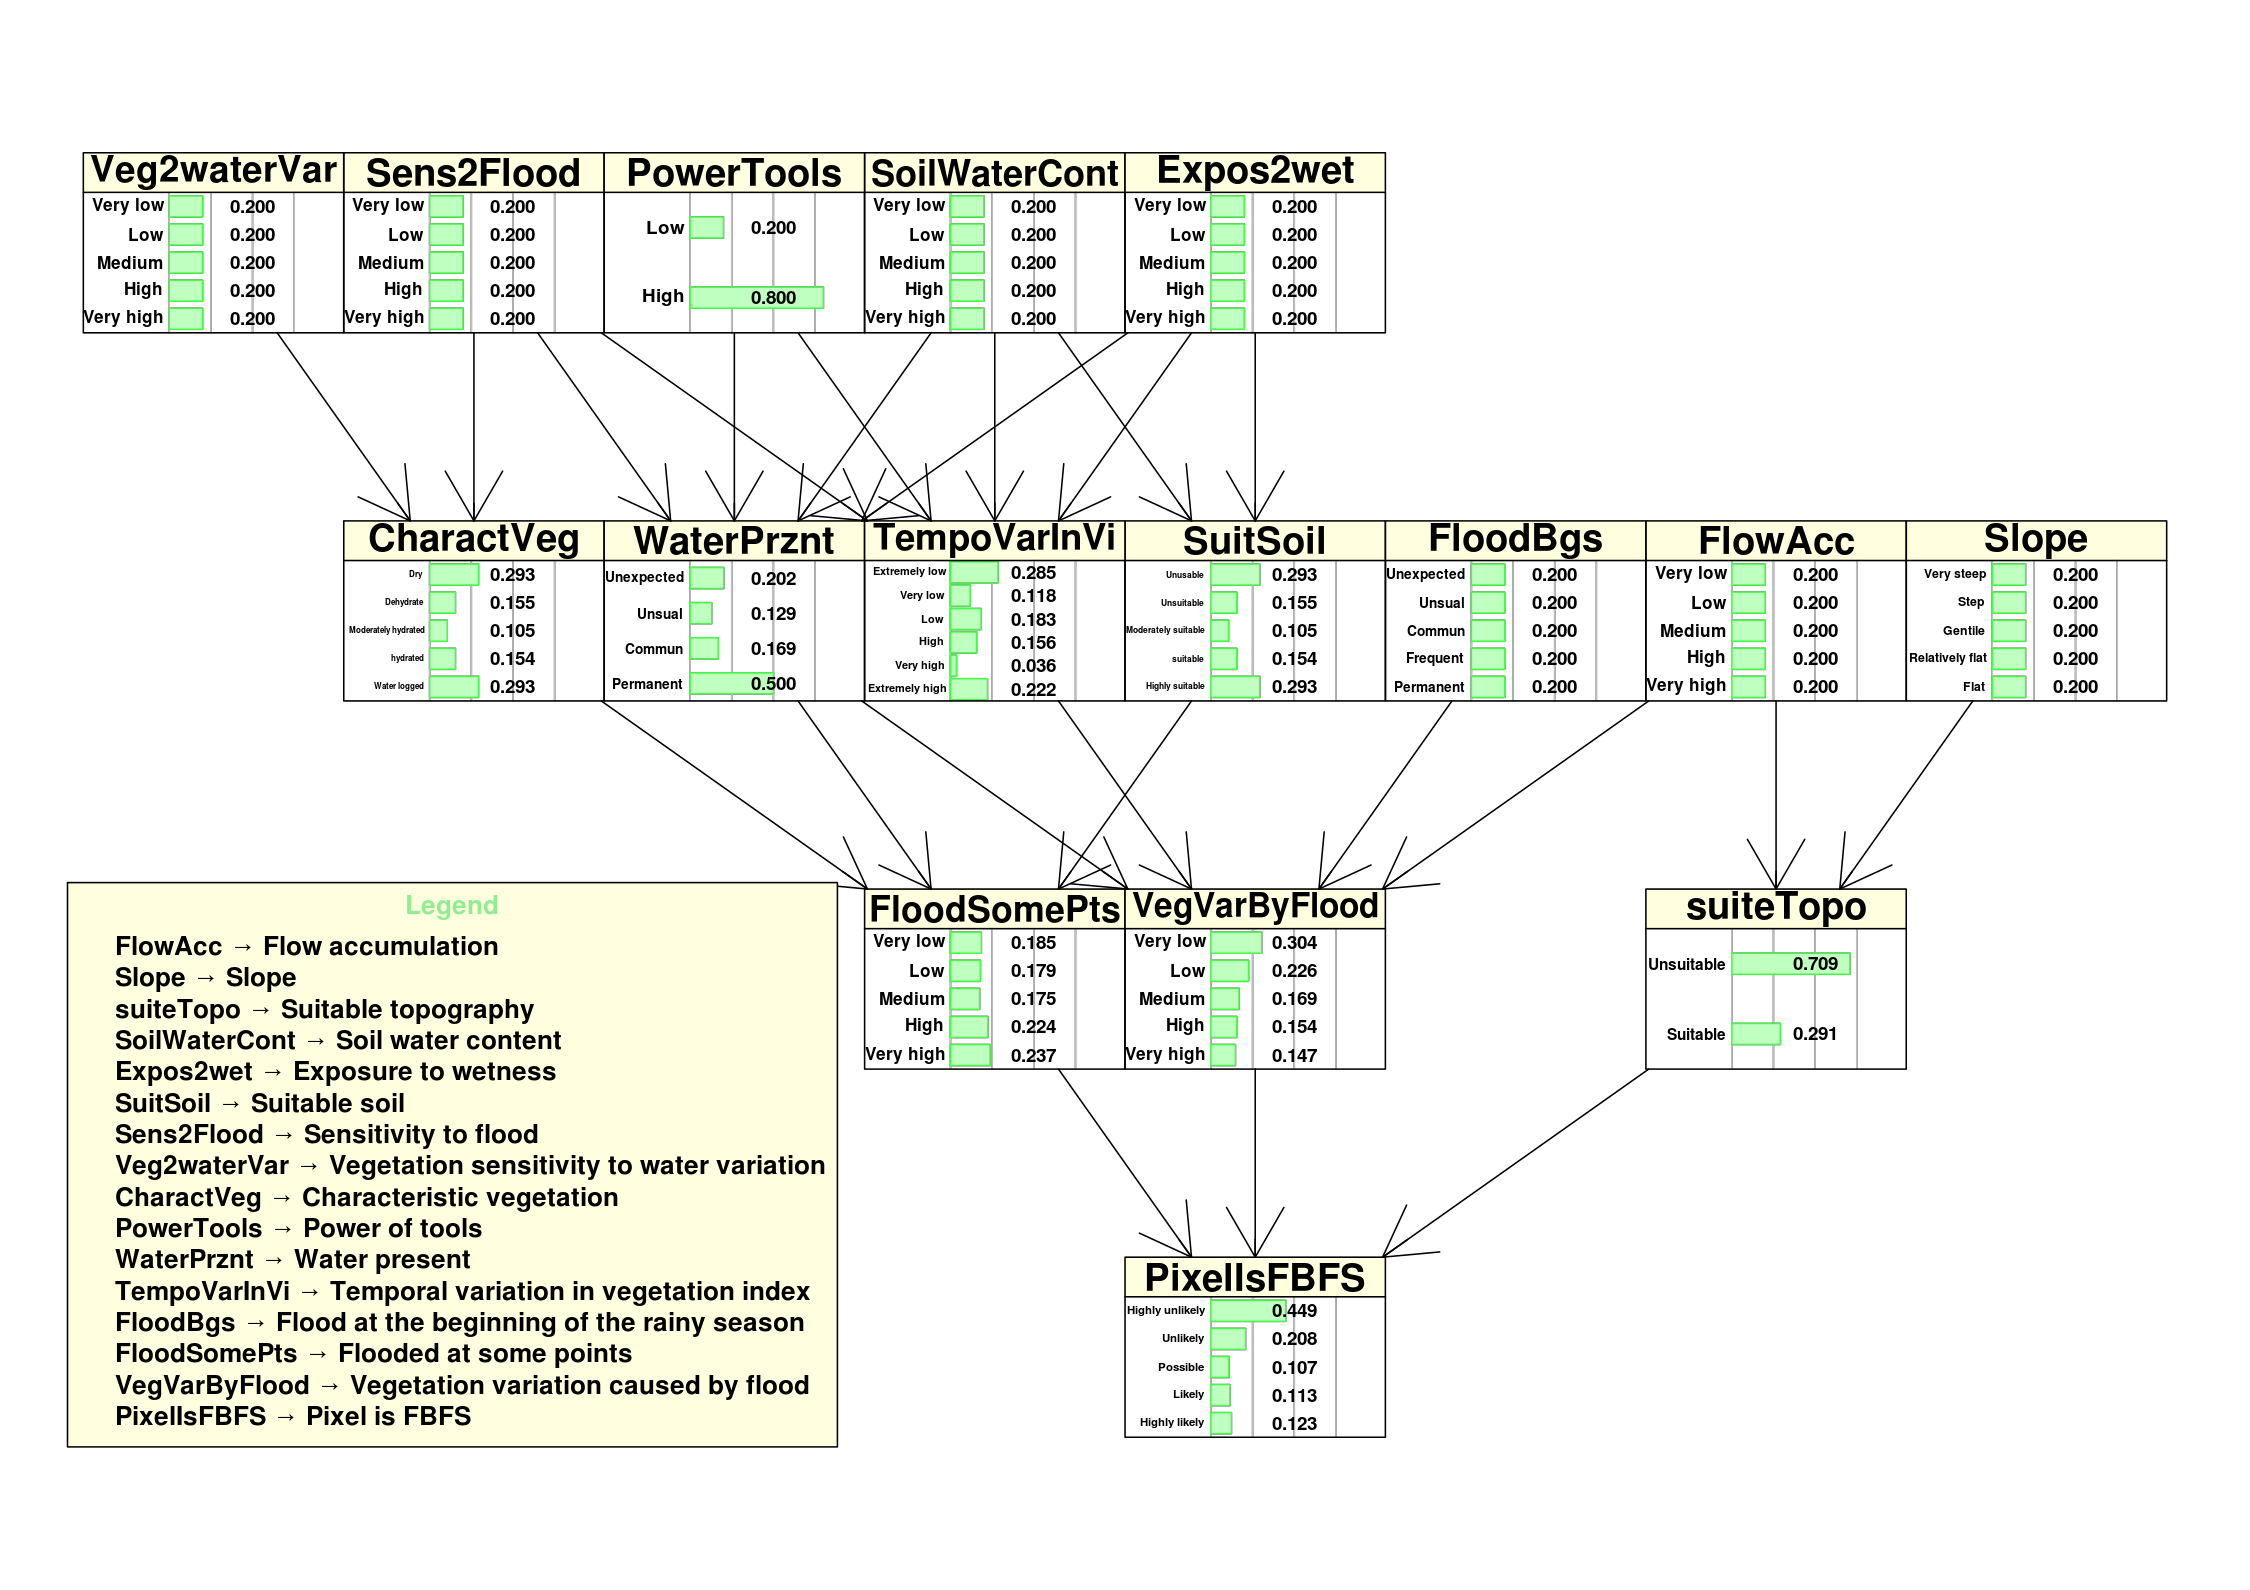
\includegraphics[width=1\linewidth]{figures/Mapping_FBFS_bayesian_network} \caption{Bayesian Network describing the causal reasoning used for mapping FBFS in Kisumu, Kenya.}\label{fig:fig1}
\end{figure}

The topographic suitability of a pixel (suiteTopo) depends largely on its slope (Slope) and the number of pixels draining into it (FlowAcc). While the accumulation of flow (FlowAcc) is important to the amount of flood reaching the pixels, it is rather the slope (Slope) and the gravity that determine whether the water will be kept or transmitted by that pixel.

The extent to which vegetation variation is caused by flood water (VegVarFlood) can be a straightforward indicator for mapping flood-based agriculture but also difficult to measure. Vegetation variation caused by flood (VegVarFlood) was therefore assessed via proxy variables. For the temporal variation in vegetation indices (TempoVarInVi) to be attributed to flood to some extent (VegVarFlood) at given pixel, one may expect a certain degree of flow accumulation (FlowAcc), and a certain likelihood of flood events near the beginning of the growing season (FloodBgs). Then, the temporal variation in vegetation (TempoVarInVi) of the pixel is assumed to be influenced by a number of factors such as its soil water content (SoilwaterCont), its exposure (Expos2wet) and sensitivity to flood (Sens2Flood), or even the quality of the data in relation with the type of algorithm used in processing these data (PowerTools).
For a given pixel to be flooded at some points (FloodSomePts), there must be water presence either on the ground (WaterPrznt). This is moderated by the soils suitability (SuitSoil) resulting in specific type of vegetation (CharactVeg). Therefore, the extent to which a pixel is flooded (FloodSomePts) can be deduced from its typical vegetation (CharactVeg), the soil suitability (SuitSoil), and the presence of water (WaterPrznt). Soil suitability to FBFS is defined by its exposure to wetness (Expos2wet) and more importantly its water content (SoilWaterCont). Water presence (WaterPrznt) may depend on soil water content (soilWaterCont), the power of tools (PowerTools), and the sensitivity to flood (Sens2Flood). Characteristic FBFS' vegetations are assumed to be due to vegetation sensitivity to water variation (Veg2waterVar) and the sensitivity of the area to flood (Sens2Flood).

\hypertarget{I32}{%
\subsubsection{The shapefiles data}\label{I32}}

The shapefiles of the study areas were acquired from the global administrative boundaries database\textsuperscript{\protect\hyperlink{ref-GADM_2018}{45}} as level 1 product, using the string country name as argument to \texttt{getData} function from the raster package,\textsuperscript{\protect\hyperlink{ref-Hijmans_2019}{46}} from which we extracted the shapefile of the area of interest. These shapefiles were latter used to identify the MODIS H/V titles corresponding to the area. Other shapefiles used are the spatial polygons representing well known selected surface features (land use/ land cover) used to understand the behaviour of the spectral response in the area. These were either collected during fields works using handheld GPS devices or digitized on Google Earth to be used to query the spectral response of pixels they match spatially. The surfaces features considered here include different depth water bodies, settlements, FBFS fields, rainfed agricultural fields, riparian forests, forests with varying degree of density, and sugarcane fields having relatively extended growing season.

\hypertarget{I33}{%
\subsubsection{MODIS Tera}\label{I33}}

We considered a period of three years (2014 - 2016) and queried all available MODIS Tera data overlapping the acquired shapefiles of the area of interest (section \ref{I32}). We first determined the Horizontal and Vertical tiles corresponding to the spatial coverage of the shapefiles and used these to define the appropriate geo-locations of the study area relative to the MODIS Sinusoidal grid systems using the \texttt{getTiles} function from the MODIS package.\textsuperscript{\protect\hyperlink{ref-Mattiuzzi_and_Detsch_2018}{47}} As result, the Kisumu County falls in-between the h21v09 and h21v08. Based on these tiles and the temporal window of interest, we mosaiced the images and calculated the NDSIs after filtering and downloading the data from MODIS global online database (i.e.~LP DAAC, LAADS) using the machine-to-machine routines embedded in the \texttt{MODIStsp} function from the package of the same name.\textsuperscript{\protect\hyperlink{ref-Busetto_and_ranghetti_2016}{48}} Since the MODIS data are provided in hierarchical data format (hdf), they were re-projected to World Geodetic System 1984 (WGS 84) and subsequently translated into Geotiff format using GDAL 2.2.3.\textsuperscript{\protect\hyperlink{ref-GDAL_OGRcontributors_2018}{49}}

\hypertarget{I4}{%
\subsection{Making sense of data in the context}\label{I4}}

\hypertarget{I41}{%
\subsubsection{Phenological overview of the landscape texture}\label{I41}}

We sampled approximatively 40\% of pixels considering a regular grid sampling using the \texttt{spSample} function from the sp package.\textsuperscript{\protect\hyperlink{ref-Bivand_et_al_2013}{50},\protect\hyperlink{ref-Pebesma_Bivand_2005}{51}} These time series of NDSIs were examined using boxplots. The NDSIs considered include the Normalized Difference Vegetation index,\textsuperscript{\protect\hyperlink{ref-Rouse_et_al_1973}{30},\protect\hyperlink{ref-Tucker_1979}{33}} the Normalized Difference Flood index,\textsuperscript{\protect\hyperlink{ref-Boschetti_et_al_2014}{10}} the Goa's Normalized Difference Water index,\textsuperscript{\protect\hyperlink{ref-Gao_1996}{25},\protect\hyperlink{ref-Ji_et_al_2009}{28}} and the mcfeeters' NDWI.\textsuperscript{\protect\hyperlink{ref-Ji_et_al_2009}{28},\protect\hyperlink{ref-McFeeters_1996}{29}} These NDSIs were chosen due to their suitability in describing water and vegetation.\textsuperscript{\protect\hyperlink{ref-Boschetti_et_al_2014}{10},\protect\hyperlink{ref-Gao_1996}{25},\protect\hyperlink{ref-Ji_et_al_2009}{28},\protect\hyperlink{ref-McFeeters_1996}{29},\protect\hyperlink{ref-Tucker_1979}{33}}

\hypertarget{I42}{%
\subsubsection{Spatio-temporal patterns}\label{I42}}

The boxplots were supported with further principal components analysis\textsuperscript{\protect\hyperlink{ref-Mardia_et_al_1979}{52},\protect\hyperlink{ref-Pearson_1901}{53}} using a customized version of the \texttt{rasterPCA} function from the RStoolbox package\textsuperscript{\protect\hyperlink{ref-Leutner_et_al_2019}{54}} making used of the \texttt{prcomp} function from the base package\textsuperscript{\protect\hyperlink{ref-RCoreTeam_2018}{35}} and other low-level functions from the raster package.\textsuperscript{\protect\hyperlink{ref-Hijmans_2019}{46}} The PCA, used to interpret the large dataset by creating a smaller number of components, was followed by other probabilistic estimations (see section \ref{I5}) defining the spatial representations of the spatial data node states to be used in the BNs. These supporting analyses focus only on the NDVI and NDFI but a comparative analysis connecting all the NDSIs across the main land uses is provided. The outputs were presented on the map to give insights on how the states of vegetation and water are spatially distributed. PCA allowed us to meaningfully interpret the large dataset by creating a smaller number of components.

\hypertarget{I5}{%
\subsection{Derivation of spatial data nodes}\label{I5}}

\hypertarget{I51}{%
\subsubsection{General Procedure}\label{I51}}

\hypertarget{I511}{%
\paragraph{Time series data}\label{I511}}

The boxplots and the comparative analysis of the NDSIs shows different patterns but these can only be hardly separated making it difficult to threshold the different NDSIs across land use / land cover. An approach based on rigid thresholding was clearly not the best option to demarcate the nature of the spectral response, at least not without making complicated statistical assumptions. A simpler way would be to approach the problem using imprecise quantifiers where fuzzy logic can be used in forms of Likert-type scales\textsuperscript{\protect\hyperlink{ref-Likert_1932}{55}} describing the scores of the spectral responses along a range; supporting the use of BNs. We therefore make use of the different ranges of the boxplot (i.e.~lowest outliers -- lower Whisker, lower Whisker - 1st quartile, 1st quartile -- 3rd quartile, 3rd quartile - upper Whisker , upper Whisker -- highest outliers) to separate the data and estimate the probability of each pixel falling within each of these ranges at each time step in the time series (Figure 5). Although rarely use for deriving variable states, boxplot has been used in all kind of statistics for the last 40 years. Beyond their incredible simplicity, boxplots use robust statistics to summarise data in terms of five-numbers while being particularly handy when comparing the distributions of these data across groups.\textsuperscript{\protect\hyperlink{ref-Wickham_and_Stryjewski_2012}{56}}To estimate the probability for a given range, we first recoded all values outside of that range to 0 whereas the values falling within the range were recorded to 1. This way, all the real-valued time series was reclassified into presence - absence time series data. Thereafter, the final probability of a pixel belonging to a range can be easily estimated using the ratio between the presence and absence of that pixel in the range throughout the time series (eq. 1).

\[P(p_i \in range_j) = \frac{n_{p_i \in range_j}}{N}\]

(eq.1)
Where P(p\_(i ϵ 〖range〗\emph{j ) ) is the probability of the pixel i belonging to the range j, n}(p\_i ϵ 〖range〗\_j ) is the number of time the pixel i belonged to the range j, and N is the sample space (total size of the time series).

After estimating the probabilities for each boxplot range, these ranges were mapped into fuzzy linguistic quantifiers in forms of low, medium, high etc. (depending on the number of states identify by the boxplot algorithm) to provide vegetation states in a spatially explicit manner. For example, in situation where all the five boxplot ranges are present, lower outlier values were mapped to very low, the lower Whisker to low, the interquartile range to medium, the upper Whisker to high and the upper outliers to very high. These states, computed in separated raster layers, were then merged into one single layer to provide discrete states on which the Bayesian network can be easily operationalized.

The decision to assign a state value to a given pixel was made transparently using fully probabilistic heuristics in 3 sequential steps. The first step consisted in assigning a particular state to a given pixels if that state scored the highest probability and only if that highest probability is exclusive. Thus, all cases where 2 or more highest probability co-exist are considered as unknown and ignore until the second step. Such cases having equal probability states were commonly encountered at the edges where two consecutive states spatially meet. In the second step, these confusing pixels having 2 or more maximal probability of state occurrence are filled in using majority rule. Herein, since spatial feature are geographically auto-correlated in general, we applied a 3 by 3 moving window (eight-way connectedness) centred on each of these uncertain state value pixels and estimate their state value based on the values of the 8 neighbourhood pixels. Similarly, to the first step, a particular value among the values of the 8 neighbours is chosen when and only when it is the only value that occurs the most. Whenever 2 or more states happen to be the most probable at the same time, the pixel is left out and handled at the third step. In the third step, the rest of these confusing pixels, where the first and second steps heuristics failed, were modelled using decision tree recursive partitioning classification algorithm. We first extracted the maximal values which correspond to the highest probability across all these remaining confusing pixels to fit a classification regression tree (CART) model and used that model to conditionally infer their state values. Therefore, after this third step all pixel state value were estimated, and the resulting raster can be used as spatial data node in the BNs model. The boxplot statistics were computed using our own defined function based on \texttt{boxplot.stats} function from the grDevices package.\textsuperscript{\protect\hyperlink{ref-RCoreTeam_2018}{35}} We used the \texttt{reclassify} and the \texttt{calc} functions both from the raster package\textsuperscript{\protect\hyperlink{ref-Hijmans_2019}{46}} to recode the pixel values and to estimate the probability respectively. The second step confusing pixels were handled using \texttt{modal} function from within the \texttt{focal} function also from the raster package.\textsuperscript{\protect\hyperlink{ref-Hijmans_2019}{46}} The CART model was fitted using the \texttt{ctree} function from the party package\textsuperscript{\protect\hyperlink{ref-Hothorn_et_al_2006}{57}} whereas the third step confusing pixels' inference was achieved by supplying an anonymous function wrapping the \texttt{predict} function from the stats package\textsuperscript{\protect\hyperlink{ref-RCoreTeam_2018}{35}} as argument to \texttt{calc} function.\textsuperscript{\protect\hyperlink{ref-Hijmans_2019}{46}}

\hypertarget{I512}{%
\paragraph{Single layer data}\label{I512}}

In the case of single layer data where time series does not make sense (e.g.~slope and flow accumulation) or where nodes were derived from times series as single layer (e.g.~exposure to wetness, vegetation sensitivity to water), a slightly different procedure compared to that adopted for time series data (section I5) was adopted for Bayesian network nodes making. We rather used the boxplot's five-numbers approach in a much straightforward way by exploiting the spatial variability across cell values since the temporal component of this variability no longer exists. We first extracted all pixel values and computed the five-numbers from which ranges corresponding to discrete states were computed. These ranges were then directly recoded into unique values mapping to fuzzy linguistic quantifiers. The process is somewhat a simple raster reclassification task except that the reclassification matrix was derived directly from the natural breaks of the data.

\hypertarget{I52}{%
\subsubsection{Specific procedure}\label{I52}}

\hypertarget{I521}{%
\paragraph{Soil water content}\label{I521}}

The node soil water content, as it says, estimates the probability of water in soil and is therefore related to soil water holding capacity. This was computed as a composite index by aggregating the NDII6,\textsuperscript{\protect\hyperlink{ref-Hunt_and_Rock_1989}{26}} the NDII7,\textsuperscript{\protect\hyperlink{ref-Hunt_and_Rock_1989}{26}} the NDVI,\textsuperscript{\protect\hyperlink{ref-Tucker_1979}{33}} and the NDFI.\textsuperscript{\protect\hyperlink{ref-Boschetti_et_al_2014}{10}} While the NDII6 and the NDII7 perform well in detecting a mixture in different compartments (e.g.~plant water, soil water, open water etc.) due to the presence of NIR and SWIR bands, the NDFI gives an estimate of flood conditions whereas the NDVI assesses the presence and condition of vegetation. Combining these in one composite index may provide a powerful tool for ecological studies since one index can be extracted from another to provide a new metric.\textsuperscript{\protect\hyperlink{ref-Boschetti_et_al_2014}{10}} For example, knowing that the NDII6 broadly assess soil and vegetation water content, one could extract the NDVI to estimate the soil water content. Likewise, the NDFI can be extracted to provide an estimate of vegetation water content. We used such assumption to estimate the soil water content using the eq. 2. Such tricks where the original meaning of an index is altered by subtracting another index is commonly used in remote sensing and is by far the back bone of the spectral index theory.
\[SWC_i = \frac{1}{2}\times ( \sum_{i=1}^{n} NDII6_i + \sum_{i=1}^{n}NDII7_i + 2\times \sum_{i=1}^{n}NDFI_i - 2\times \sum_{i=1}^{n}NDVI_i )\] (eq.2)
Where SWCi is the soil water content, and n the total length of the time series.

For each of these 4 indices, we first computed the total over the time series. This is meant to estimate the total value scored in whatever the index measures. For example, we assumed that the sum of the NDFI values over the period of the 3 years considered in this study at a given pixel gives an estimate of the total water received by that pixel. After computing these total values scored, we then proceeded by summing-up the total value scored by the NDII6 and the NDII7 from which we extracted twice the total value scored by the NDFI. From the resulting value, we then extracted twice the total value scored by the NDVI (eq. 2). The idea is to reduce the influence of vegetation water from a total of water contained in soil and vegetation. So doing, the remaining water would mainly be due to the above and below-ground soil water. These estimates were improved by adding to each the scored value of the NDFI which is another way to estimate soil wetness. We used both the NDII6, the NDII7 and the NDFI because to take the advantage of the potential of the SWIR spectral domain as much as possible. This, however, is equivalent to doubling the real overall potential of the water content. To account for this effect, half this value was considered after reducing the amount of water stored in vegetation which was done by subtracting twice the NDVI to account for the influence of this vegetation water in both the NDII6 and the NDII7 (eq. 2).

\hypertarget{I522}{%
\paragraph{Exposure to wetness}\label{I522}}

This node estimates the expected total water for each cell. It was computed simply as the sum of the NDFI over the time series for each pixel. In this regard, it expresses the degree to which each pixel is relatively expose to surface water wetness. It is slightly different from the soil water content in the sense that it does not account for vegetation. Literally, this is mostly the surface soil water availability / potential regardless of whether it is used or not by vegetation. We postulate that a certain amount of water may be detected at a given pixel at some point in time without being sustained since it can runoff throughout porous soils shortly or stagnate nearly permanently under saturated or impermeable soils. Contrastingly, under soils with good water holding capacity, a relatively small amount of water can be sustained for a relatively longer period. This implies that the node exposure to wetness is more concerned about the hydrology than the actual agronomy although water exposure can be a good indicator of vegetation. It is, nonetheless, important to keep in mind that vegetation is almost always incompatible with permanently water-logged areas.

\hypertarget{I523}{%
\paragraph{Sensitivity to flood}\label{I523}}

The node sensitivity to flood is computed as the absolute standard error of the NDFI to estimate somewhat how fast the flood index is changing throughout the time series. This node describes the relationship between water and soil. Supposing that all soil surface water originates from rainfall, and considering that this rainfall is relatively locally constant, then the local spatial variability in wetness can be explained by the relationship between soil (including land cover and topography) and water. For example, from remote sensing point of view, dry but flood-prone soils are likely to be more sensitive to torrential rainfall event compared to permanently saturated and water-logged soils.

\hypertarget{I524}{%
\paragraph{Vegetation sensitivity to water variation}\label{I524}}

This node was also estimated as a composite index taking into account both the NDFI and the NDVI. Flood followed by a rapid increase in vegetation has been used as indicator for mapping FBFS-like areas such as flooded rice.\textsuperscript{\protect\hyperlink{ref-Boschetti_et_al_2014}{10}} The node describes the relationship between water and vegetation using the ratio between these 2 metrics. For a given pixel, the idea conveyed by this node is simply the proportion of vegetation scored relative to amount of water received. Thus, it also implicitly gives an idea of the soil conditions because a pair of low value NDVI (absence of vegetation) and high value NDFI (water presence) may imply the presence of encrusted or swampy soils where vegetation may be sensitive to water variation.

\hypertarget{I525}{%
\paragraph{Power of tools}\label{I525}}

The power of tools was estimated from the generic product quality assessment MODLAND-wide QA bands for each pixel and date in the time series. The MODLAND-wide QA provides a general and consistent assessment of the quality (usability and usefulness) of the MODIS products to inform the user on the quality, hence, the extent to which the results of any analysis is to be appreciated. Many artefacts (e.g.~aerosol loading, cloud, data processing algorithms, sensors failure, view angle, etc.) can introduce errors or uncertainties in remote sensing data, and it is therefore advised to consider such aspects prior to their use for subsequent analysis. While the power of tools can be estimated using band specific quality assessment, we choose to use the MODLAND-wide QA which includes most of the artefacts in the assessment.

\begin{longtable}[]{@{}lll@{}}
\caption{Translation of 2-bit pixel level-QA in MODLAND.\textsuperscript{\protect\hyperlink{ref-Roy_et_al_2002}{58}}}\tabularnewline
\toprule
2-bit encoded per pixel QA code & Decimal value & Quality attribute meanings\tabularnewline
\midrule
\endfirsthead
\toprule
2-bit encoded per pixel QA code & Decimal value & Quality attribute meanings\tabularnewline
\midrule
\endhead
00 & 0 & Pixel produced, good quality, not necessary to examine more detailed QA\tabularnewline
01 & 1 & Pixel produced, unreliable or unquantifiable quality, recommend examination of more detailed QA\tabularnewline
10 & 2 & Pixel not produced due to cloud effects\tabularnewline
11 & 3 & Pixel not produced primarily due to reasons other than cloud\tabularnewline
\bottomrule
\end{longtable}

In the MODLAND-wide QA framework, four quality states are possible (Table 1) and the power of tools was estimated as the probability of being wrong accordingly. For each pixel throughout the time series, we remained sceptical to values greater than zero in Table 1 and the probability of being wrong was computed by dividing the count of these values by the total length of the time series. The resulting raster layer was then discretised to provide the node to be used in the BNs following the procedure described in section \ref{I512}. It is worth noting that most of the poor qualities are concentrated around water bodies, hence the node power of tools was used for dual purpose in the causal model despite the little spatial variability.

\hypertarget{I526}{%
\paragraph{Slope and Flow accumulation}\label{I526}}

Many approaches and algorithms for deriving hydrologic information from topography have been proposed in diverse conceptual forms with each having its strengths and limitations;\textsuperscript{\protect\hyperlink{ref-Arge_et_al_2003}{24},\protect\hyperlink{ref-Jenson_and_Domingue_1988}{27},\protect\hyperlink{ref-Tarboton_1997}{59}} mostly relying on what is known as the 3 steps conditioning procedures.\textsuperscript{\protect\hyperlink{ref-Arge_et_al_2003}{24},\protect\hyperlink{ref-Jenson_and_Domingue_1988}{27}} DEM conditionings are commonly used as prerequisites for computing various topographic structures such as upslope areas, specific catchment areas, girded networks or flow paths and are extensively discussed in the literature.\textsuperscript{\protect\hyperlink{ref-Arge_et_al_2003}{24},\protect\hyperlink{ref-Jenson_and_Domingue_1988}{27},\protect\hyperlink{ref-Tarboton_1997}{59},\protect\hyperlink{ref-OCallaghan_Mark_1984}{60}} These are the filling of depressions in the original DEM, the derivation of flow directions and the computation of flow accumulation. In this paper, these were derived using TauDEM software version 5.3\textsuperscript{\protect\hyperlink{ref-Yang_et_al_2006}{34},\protect\hyperlink{ref-Tarboton_1997}{59},\protect\hyperlink{ref-Tarboton_et_al_1991}{61},\protect\hyperlink{ref-Tesfa_et_al_2011}{62}} from within R. Routines were sent via system calls from R to TauDEM and throughputs are routed from TauDEM to R to be further processed to discrete raster data following the single layer procedure described in section \ref{I512}. TauDEM routines along with the conceptual and algorithmic details on the DEM conditioning are beyond the scope of this paper. The reader is referred to TauDEM website and related literature.\textsuperscript{\protect\hyperlink{ref-Arge_et_al_2003}{24},\protect\hyperlink{ref-Jenson_and_Domingue_1988}{27},\protect\hyperlink{ref-Tarboton_1997}{59},\protect\hyperlink{ref-Tarboton_et_al_1991}{61}--\protect\hyperlink{ref-Wallis_et_al_2009}{63}}
The original void-filled SRTM DEM (section \ref{I21}) was used in the 3 steps normative conditioning procedure\textsuperscript{\protect\hyperlink{ref-Jenson_and_Domingue_1988}{27}} to compute the slope and flow accumulation layers to account for the corresponding spatial data nodes in the BNs as described in section \ref{I31}. Our approach fully accommodates for simple and looping depressions and flat areas as suggested by Jenson \& Domingue\textsuperscript{\protect\hyperlink{ref-Jenson_and_Domingue_1988}{27}} and Tarboton.\textsuperscript{\protect\hyperlink{ref-Tarboton_et_al_1991}{61}} We computed the slope as the drop distance (tangent of the slope angle; see TauDEM website) from which we derived the D-infinity flow direction as the direction outwards water flows from that pixel based on the Single-flow-direction concept.\textsuperscript{\protect\hyperlink{ref-Arge_et_al_2003}{24},\protect\hyperlink{ref-Tarboton_1997}{59}} Based on the derived flow directions, the flow accumulation at each pixel was then calculated as the number of pixels draining into it.

\hypertarget{I527}{%
\paragraph{Water presence}\label{I527}}

The water presence node estimates the likelihood of encountering water on the ground given the 3 years times series considered in this study. Flood is perhaps the most important characteristic of FBFS, and therefore water signature may be captured by the sensor in these areas. We therefore used the NDFI to assess such cases across all pixels in the study area. This was done using the procedure described in section \ref{I5}.

\hypertarget{I528}{%
\paragraph{Temporal variation in vegetation}\label{I528}}

The temporal variation in vegetation was estimated as pixel level vegetation anomalies using NDVI based on an approach of vegetation phenology (Figure 2). Our approach consisted in estimating the length of the growing season from which was then extracted an average interpolated surface derived from it. This is based on the assumption that the vegetation period is relatively extended under FBFS-like settings where plants take advantages of residual moisture from previous flooding.\textsuperscript{\protect\hyperlink{ref-VanSteenbergen_et_al_2010}{2}} In this case, these FBFS may be found in areas having unusually higher growing period relative to a general spatial trend.

\begin{figure}
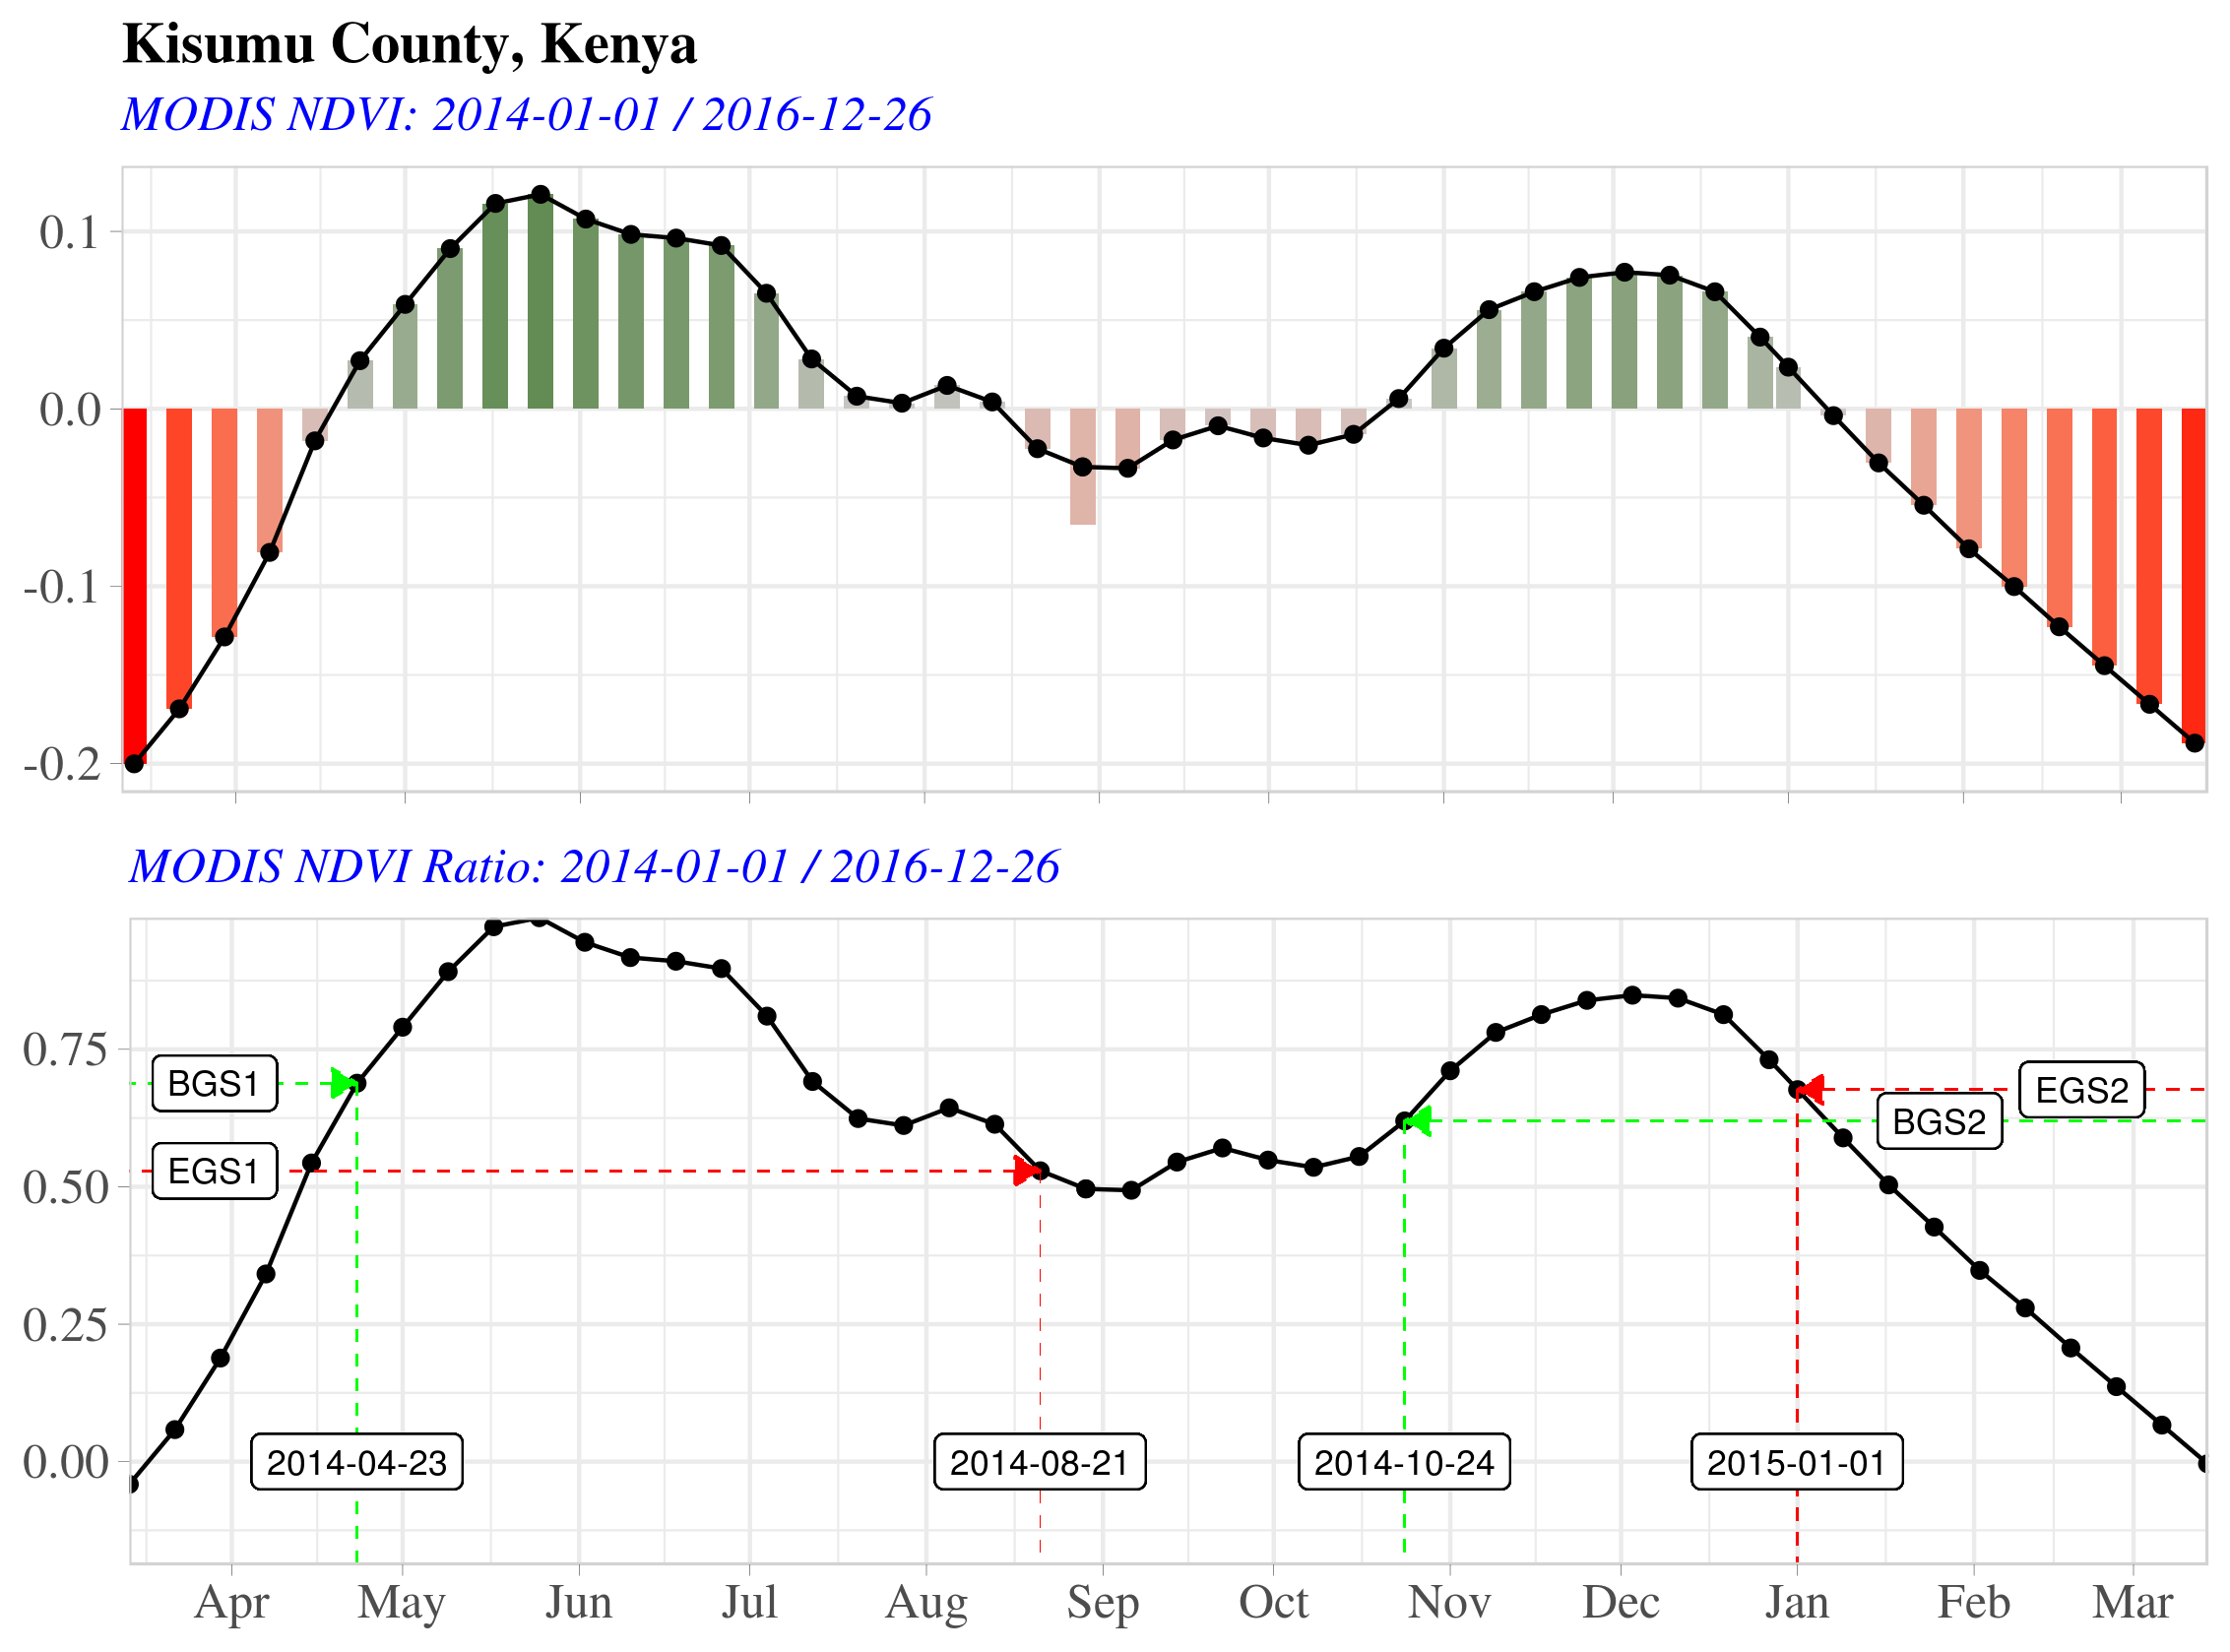
\includegraphics[width=1\linewidth]{figures/Mapping_FBFS_vegetation_seasonality} \caption{Vegetation seasonality in Kisumu County (Kenya).}\label{fig:fig2}
\end{figure}

EGS = End of growing season; BGS = Beginning of growing season; the indices (1 and 2) indicate the first and second seasons respectively.

The NDVI has been used in many ways to study vegetation phenology.\textsuperscript{\protect\hyperlink{ref-DeLeeuw_et_al_2012}{64}--\protect\hyperlink{ref-Yu_et_al_2012}{66}} We used the NDVI time series to first estimate the ratio (Figure 2) at which the vegetation density is changing throughout the year.\textsuperscript{\protect\hyperlink{ref-Yu_et_al_2010}{65}--\protect\hyperlink{ref-White_et_al_1997}{67}} The NDVI ratio was calculated using the eq. 3.\textsuperscript{\protect\hyperlink{ref-Yu_et_al_2010}{65},\protect\hyperlink{ref-White_et_al_1997}{67}}

\[NDVI_{ratio} =   \frac{NDVI-NDVI_{min}}{NDVI_{max} - NDVI_{min}}\] (eq.3)
Where NDVIratio is the NDVI ratio of the pixel throughout the time series ranging from 0 to 1, NDVI is the NDVI of that pixel at a given time step in the times series, NDVImax and NDVImin are respectively the maximal and the minimal NDVI values scored by the pixel over the time series.
The NDVI ratio (eq. 3) is consistent since its value is normalised relative to itself. This ratio was derived considering the 3 years period considered in the study whereby the minimum and the maximal values were derived according to the phenological phases (Figure 2). An NDVI ratio at a given development stage informs on the proportion of vegetation relative to the total attainable biomass regardless of the land cover type.\textsuperscript{\protect\hyperlink{ref-White_et_al_1997}{67}} While this method can help to avoid the use of locally adopted thresholds\textsuperscript{\protect\hyperlink{ref-White_et_al_1997}{67}} since a generic threshold above which the onset and cession of the rainy season can be consistently estimated, deciding which ratio value to consider as that common threshold is another question. To address this concern, we extracted the seasonal component of the time series from which individual seasons were separated. Based on the assumption that the NDVI changes rapidly in the near onset and secession of the rainy season, we then scanned each season forwards and backwards questing for possible jumps (i.e.~± 3 standard deviation) in the values of the NDVI ratio. When scanning forwards, then a jump corresponds to the onset whereas the cessation is estimated scanning backwards. After locating the dates corresponding to these onset and cessation for each cell, their difference was calculated to estimate the length of the growing season for each season. These raster layers were aggregated to 5 km2 interpolation surface using the \texttt{aggregate} function from the raster package\textsuperscript{\protect\hyperlink{ref-Hijmans_2019}{46}} to fit a thin plate spline regression model using the \texttt{Tps} function from the fields package.\textsuperscript{\protect\hyperlink{ref-Nychka_et_al_2018}{68}} The model was then used to interpolate each season using the \texttt{interpolate} from the raster package relative to the average interpolation surface.\textsuperscript{\protect\hyperlink{ref-Hijmans_2019}{46},\protect\hyperlink{ref-Nychka_et_al_2018}{68}} The anomalies were estimated as the difference between the length of the growing season and its interpolation. Finally, these anomalies were sum-up to provide a single estimate which was then discretised to provides nodes states for the Bayesian network as described in section \ref{I512}.

\hypertarget{I529}{%
\paragraph{Flood at the beginning of the rainy season}\label{I529}}

The beginning of the rainy season node was defined widely from the starting of the season to nearly the vegetation peak to account for early and late flooding. The node flood at the beginning of the rainy season, then, estimates the probability of getting flood during that critical period. Based on this assumption, we extracted, from the NDFI times series, all layers corresponding to the first 2 months from which the node states were derived using the multilayers procedure described in section \ref{I5}.

\hypertarget{II}{%
\section{Results and discussion}\label{II}}

\hypertarget{II1}{%
\subsection{Comparative profiles of the NDSIs across different surface features}\label{II1}}

\hypertarget{II11}{%
\subsubsection{Comparative behavior of the NDSIs across biomes}\label{II11}}

The temporal profile of different NDSIs across the main ecological systems is provided in Figure 3. The NDSIs seem to behave similarly across the 3 main agricultural systems (i.e.~Rainfed fields, Sugarcane fields, FBFS fields) with more pronounced flood peaks under FBFS fields. These peaks are also observed under flood-prone forests where floods seem to be seasonal. Rainfed fields seems to have more communalities (i.e.~NDSIs' scores and temporal profile) with sugarcanes fields as do FBFS fields and flood prone forest although it is hard to distinguish between these 4 biomes.

\begin{figure}
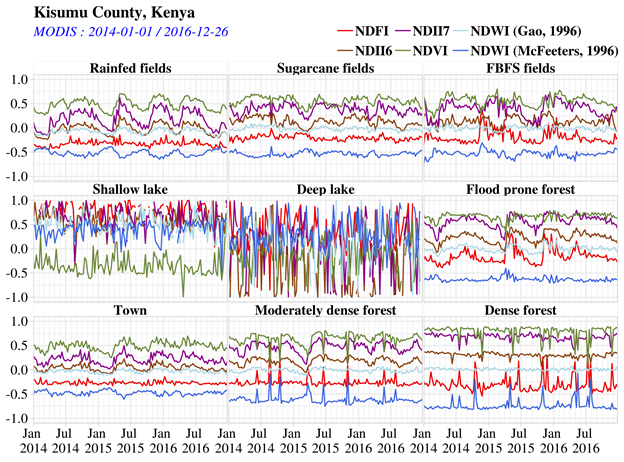
\includegraphics[width=1\linewidth]{figures/Mapping_FBFS_ndsi_comparaison} \caption{Comparative analysis and behavior of the NDSIs across different surfaces in Kisumu County (Kenya).}\label{fig:fig3}
\end{figure}

While one may expect NDFI values above 0.5 at least under FBFS fields, the 3 water-related NDSIs (including the Gao NDWI, Mcfeeters NDWI), NDFI scored negative values across the 3 different agricultural systems making thresholds specification difficult. The profile of vegetation (NDVI, NDII6, NDII7) under rainfed and FBFS fields seems to present a more pronounced seasonality contrary to sugarcane fields owing to their longer growing season resulting in moisture stability (Gao NDWI). This vegetation seasonality along with the extended length of the growing season becomes clearer under flood prone forest. Interestingly, flood prone forest seems to be different from FBFS fields with regards to vegetation density and open water stability. While both FBFS fields and flood prone forest scored positive NDVI values reaching up to 0.75, the NDVI values under flood prone forest rarely drop below 0.5 contrary to FBFS where these values can drop to 0.25. Under lakes systems (shallow and deep lakes), the signatures of the different NDSIs is rather confusing except in the case of NDVI which seems to be unique under shallow lake. While vegetation is quasi absent in littoral zone, there seems to be a permanent mixture of vegetation and water in the deep water suggesting possible Eutrophication of Lake Victoria. Forest biomes are possibly distinguishable looking at the relative scores of the different NDSIs and their temporal profiles. Flood-prone and moderately dense forests are more seasonal in vegetation than dense forests exhibiting constant moisture over time. In general, sudden drop in vegetation seems to be associated with sudden increase in water signature under both dense and moderately dense forests while no such association is observed under flood-prone forest and towns suggesting the presence of open waters that are often masked by tree canopies. While vegetation (NDVI, NDII6, NDII7) decrease from dense forest to town through moderately dense forest as expected, the opposite trend is observed with open water. Nonetheless, the soil moisture (Gao NDWI) across the 3 biomes seems to be constant. Overall, most of the NDSIs behave similarly and open water stability or the length of the growing season can be misleading in delineating FBFS fields in the area. Soil moisture (Gao NDWI) seems to be constant over time with little difference across biomes suggesting the presence of good soils for FBFS in the areas.

\hypertarget{II12}{%
\subsubsection{Comparative distribution of the NDSIs values across different surfaces}\label{II12}}

Looking at the distribution of the different NDSIs across the different biomes (Figure 4), it is clearly difficult to derive sharp threshold values for delineating most of the biomes, particularly the FBFS fields. The response of open water with regards to the different NDSIs seems to be rather odd, possibly due to the quality of the data since poor-quality data were associated with water bodies. Based the NDFI, the NDVI and the Mcfeeters' MDWI, FBFS fields can only be differentiated from shallow lake but the amount of noise is yet to be substantial considering the ranges overlapping of outliers. Considering the NDII6, the NDII7 and the Gao's NDWI, little can be done to distinguish FBFS fields from the other biomes due to the general lack statistical difference.

\begin{figure}
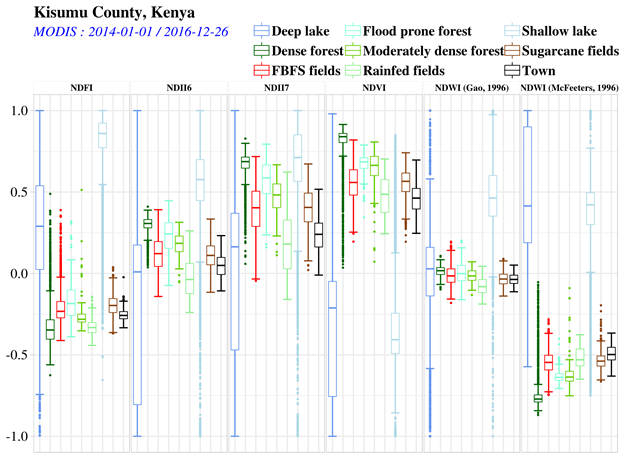
\includegraphics[width=1\linewidth]{figures/Mapping_FBFS_ndsi_accross_features} \caption{Comparative distribution of the NDSIs values across different surfaces in Kisumu County (Kenya).}\label{fig:fig4}
\end{figure}

The best statistical difference based on the NDFI seems to be between the signature of the shallow lake and the rainfed fields. However, the majority of these rainfed fields seems to experience flooding owing to their overlaps with both FBFS fields and deep lack. This is also observed with the Mcfeeters' MDWI. In a nutshell, there is redundancy in the scores of the NDSIs across the main biomes encountered in the study areas, hence they might be misleading for specifying thresholds. Consequently, there is a general lack of statistical evidence for deriving threshold values for delineating FBFS fields from the other type of ecological systems.

\hypertarget{II2}{%
\subsection{Phenological overview of the landscape texture}\label{II2}}

The average trend (represented by the interquartile range or the green medians line) depicted the phenological nature of the vegetation in the study areas with 2 annual phenological phases. The first phase seems to start from the beginning of April and ends during the period end of August -- beginning of October whereas the second starts during the period beginning of September to the middle of October and ends in the middle of March. This main trend seems to isolate the croplands in relation with rainfall seasonality in the area (Figure 5).

The Outliers seems also to describe further phenological differences in vegetation across different type of biomes in the areas. Further examination of these outliers (not shown here) as separate datasets resulted in further temporal patterns in the NDVI values which can also be seen in Figure 5 (black and red lines). The first pattern (upmost outlier in black) seems to describe relatively high vegetation spots with NDVI values ranging from 0.5 to 1 during the period February -- May. These could be due to data irregularities (sensor oversaturation during data recording, poorly corrected data, etc.) or more intuitively a sudden increase in vegetation due to the short rains in areas with relatively dense vegetation such as forests. In areas with permanent vegetation, changes in the greenness at the onset of the rainy season can be more rapid compared to agricultural fields where a certain time is required for crops to emerge and regreen the landscape. This is plausible considering that these outliers disappear when considered within the context of the upmost trend (upper whisker and upmost black line). The second pattern (lower outliers, and black line), accounting for vegetation indices in-between negative 0.25 and 0.5 seems to be positively correlated with the main pattern contrary to the third pattern (lower outliers and red line) describing vegetation indices below negative 0.25. while it is hard to tell the land use type described by the second pattern of these outliers, the third one is likely to describe water and water bodies. Overall, the study area is heterogenous and composed of several distinctive biomes with specific phenology and vegetation density, with some of these correlated over time.

\begin{figure}
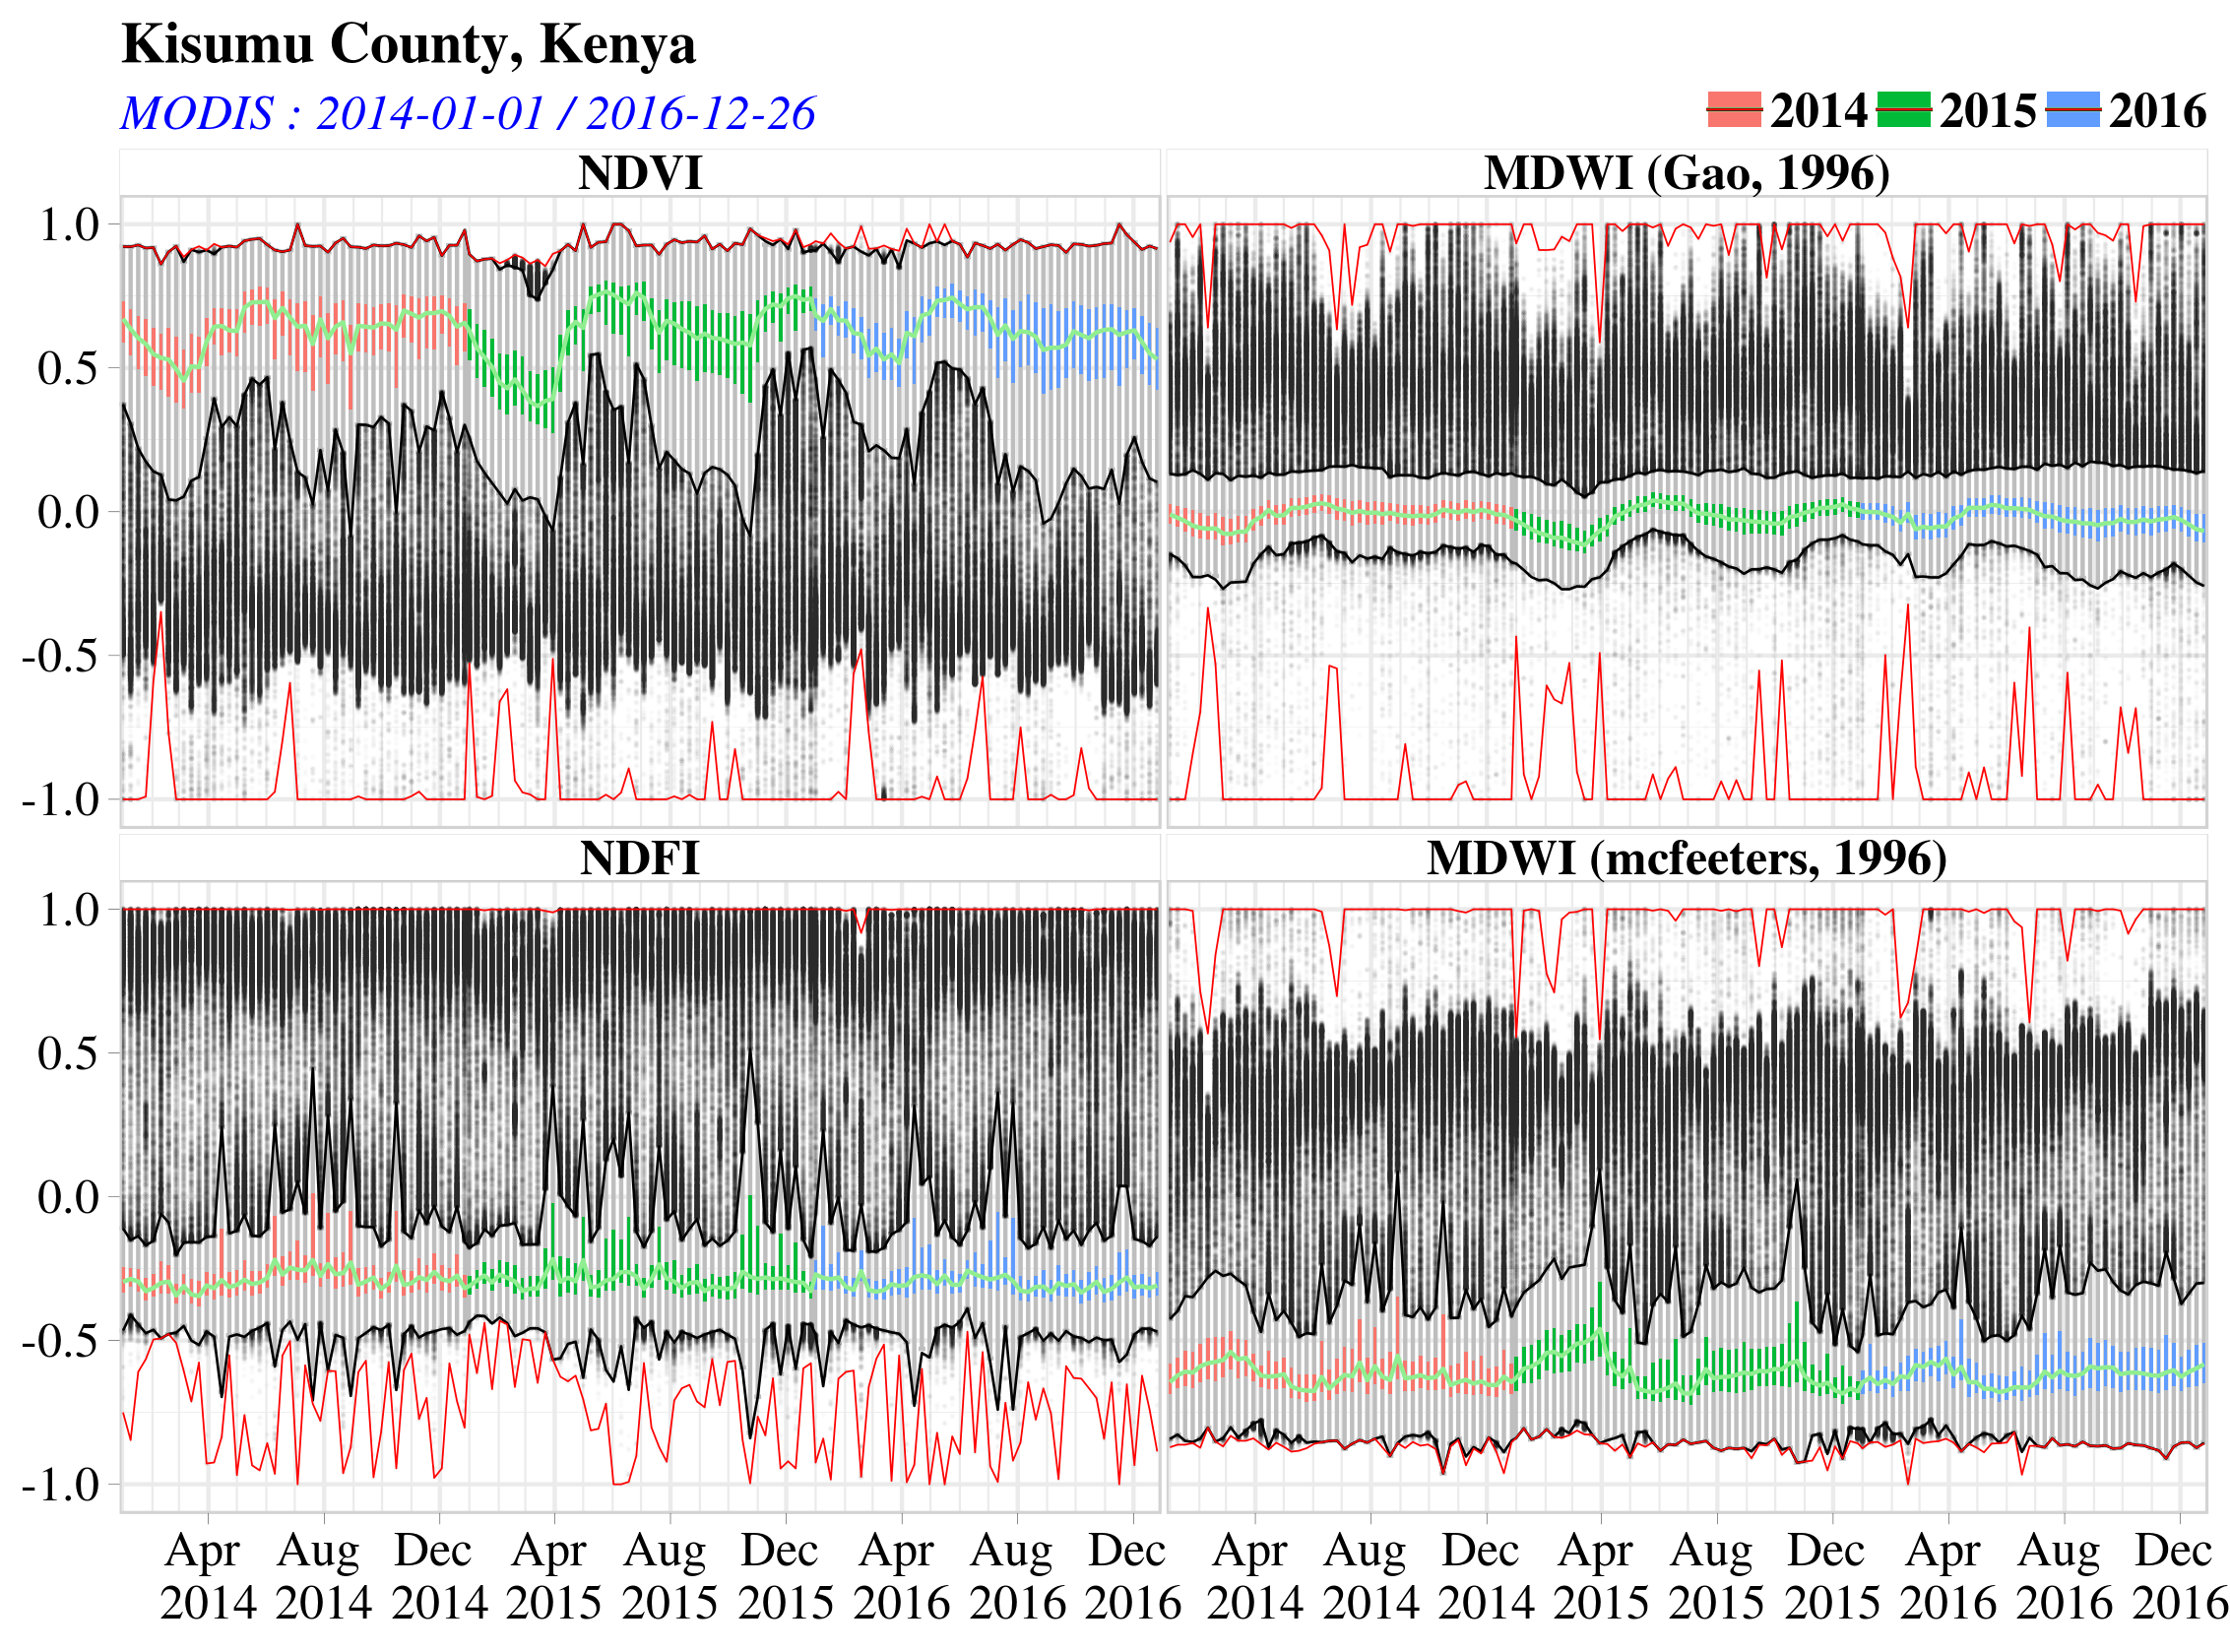
\includegraphics[width=1\linewidth]{figures/Mapping_FBFS_boxplot_temporal_variability} \caption{Boxplot of the temporal variability in water and vegetation in Kisumu county, Kenya.}\label{fig:fig5}
\end{figure}

\hypertarget{II3}{%
\subsection{Spatio-temporal variability in water and vegetation}\label{II3}}

The analysis of the NDSIs across the main existing land use / land cover provide little guidance to specify the boundaries of FBFS fields. Despite the differences in water and vegetation density (Figure 5), it was interesting to look at the main type of landscape existing in the areas and the extent to which their ecology can be appreciated in the context of seasonality. The PCA suggests that the first 3 components best describe the essential of the variability in vegetation supporting the possibility of data redundancy stated earlier (section \ref{II12}) whereas up to 13 were required for flood supporting the unpredictable nature of floods (Figure 6).

\begin{figure}
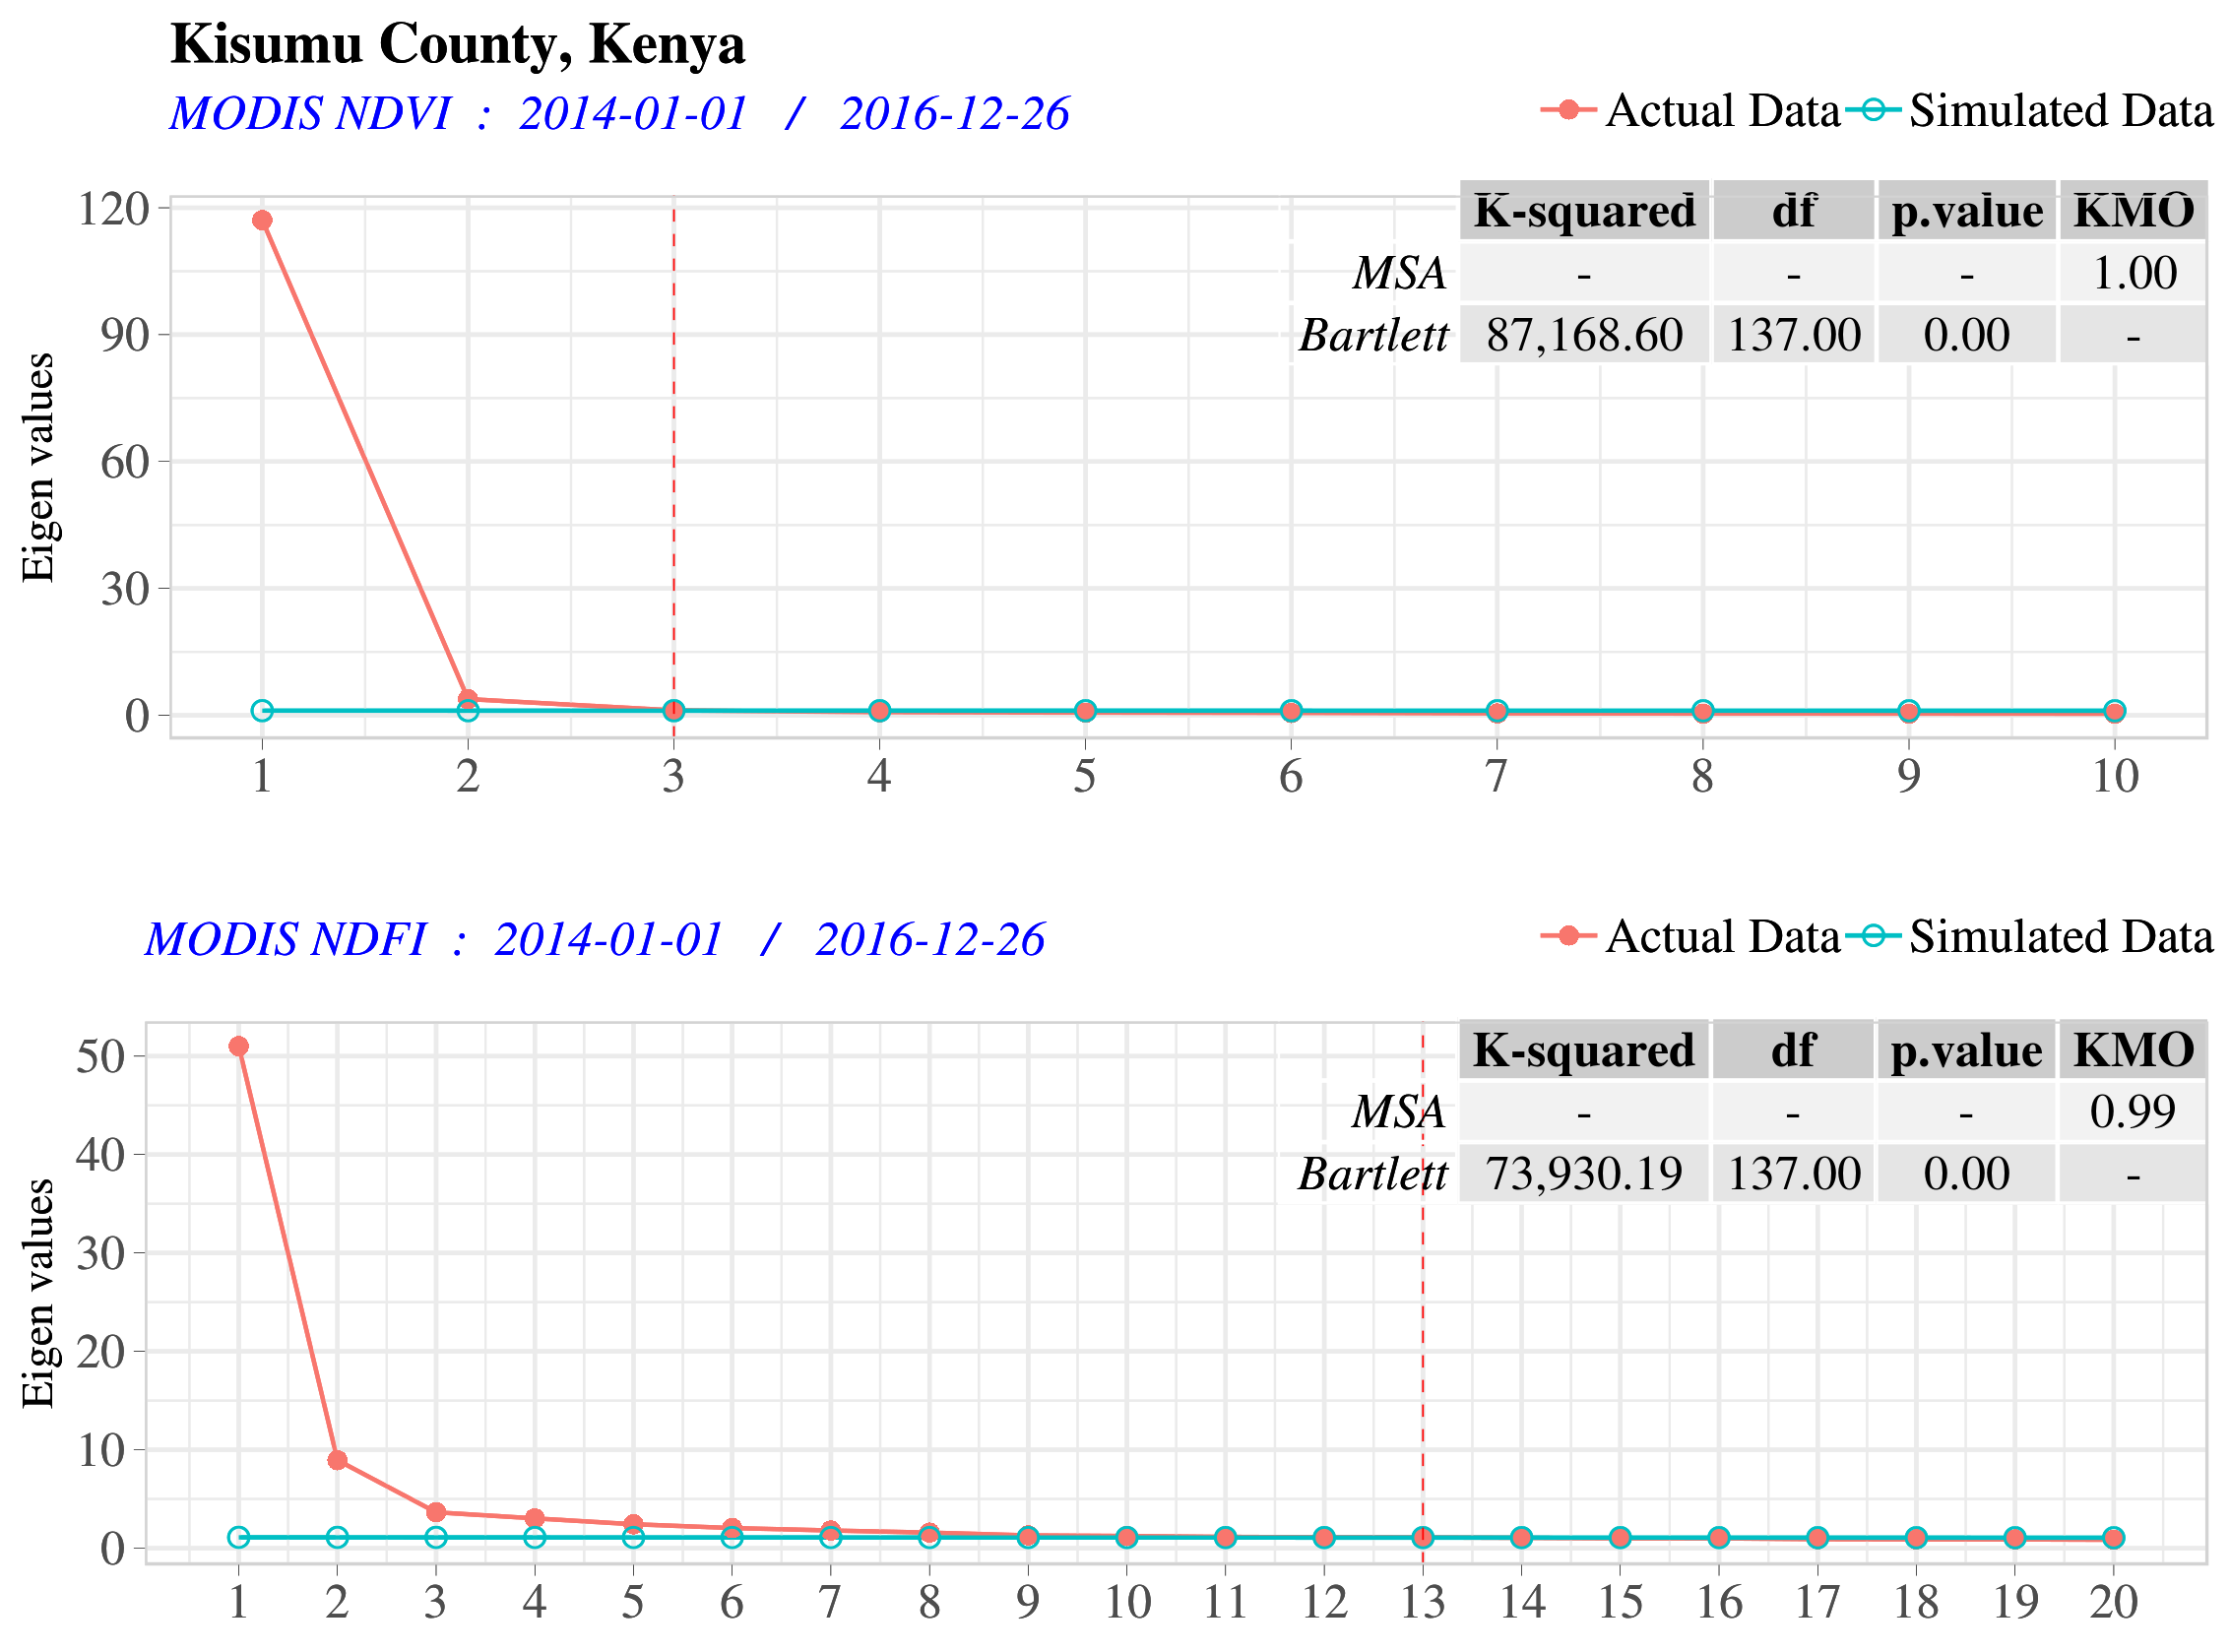
\includegraphics[width=1\linewidth]{figures/Mapping_FBFS_NDVI_NDFI_parallel_analysis_sreeplot} \caption{Scree plot of the first meaningful principal components along with the KMO and Bartlett's Test of sphericity}\label{fig:fig6}
\end{figure}

The spatio-temporal patterns of water and vegetation based on the 8 days MODIS composite in the study area presented in Figure 7 and Figure 9 respectively. The temporal variability describes the cross-pixels dominant variation over time attributed to the PCs depicted by the PCA. These are also presented as monthly aggregates to provide lumped view of the area. The Spatial patterns resulting from the scores of these PCs is also provided as maps. Based on these results,

\begin{figure}
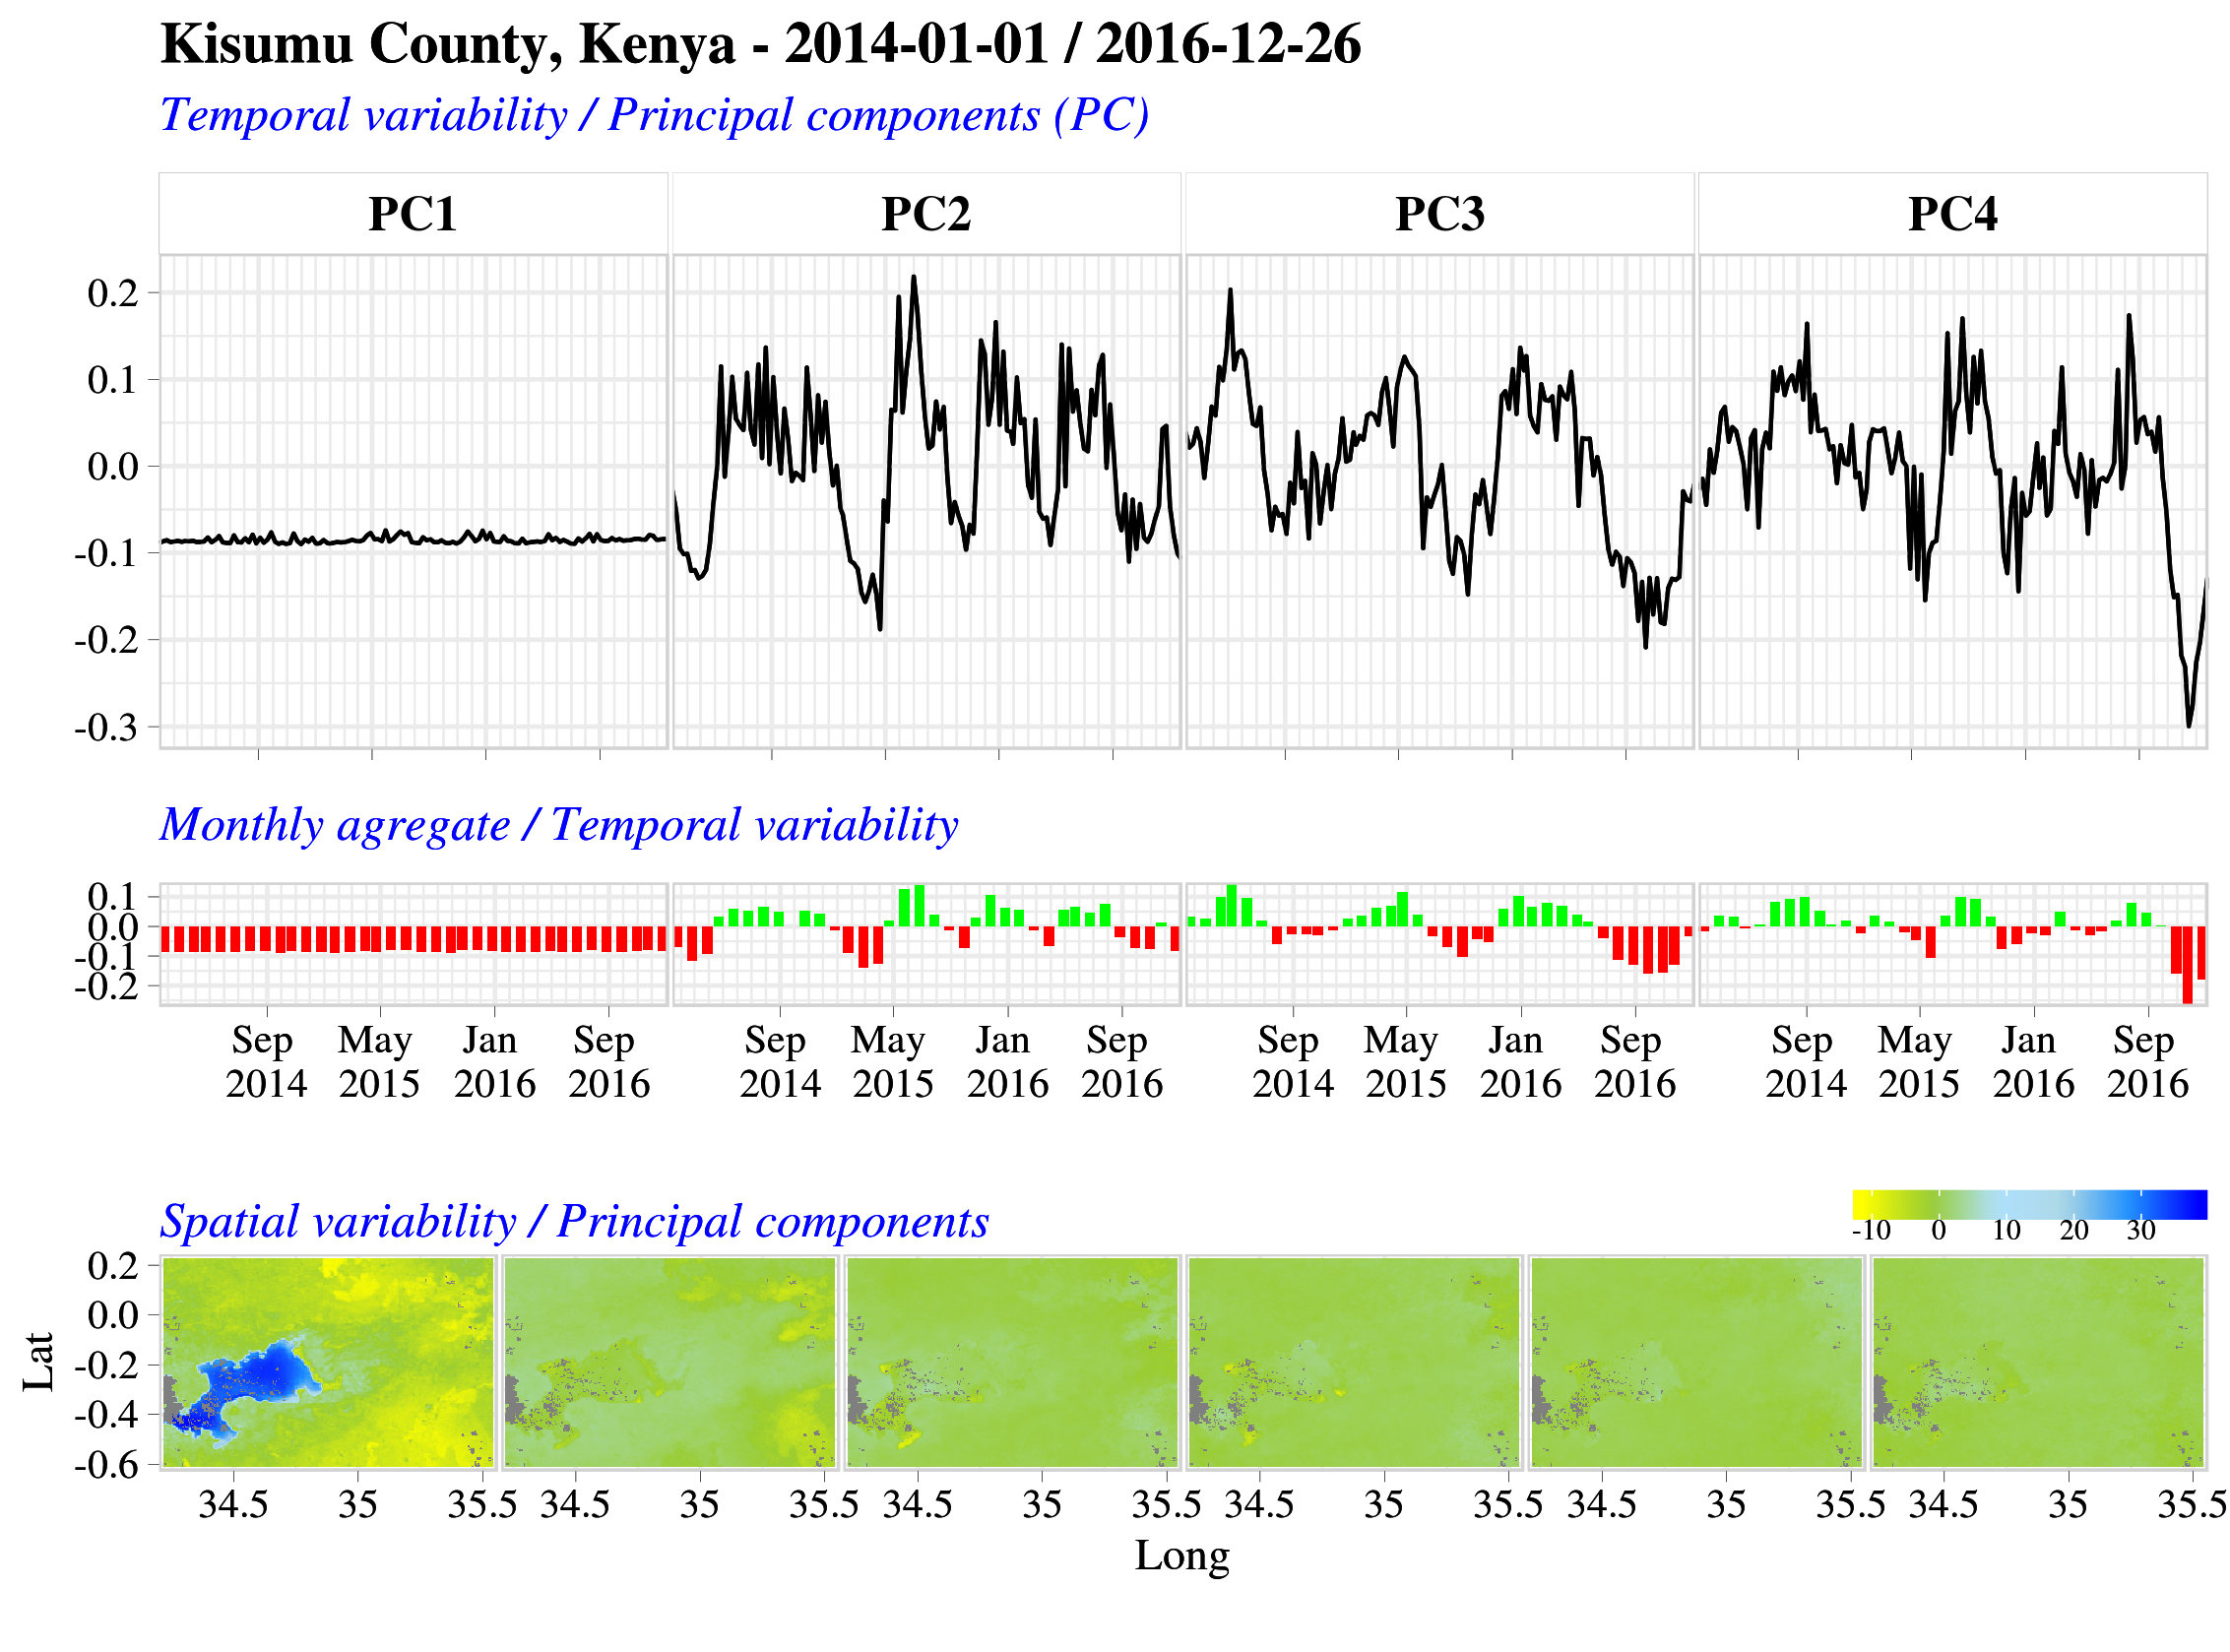
\includegraphics[width=1\linewidth]{figures/Mapping_FBFS_NDFI_PCA_plot_Kisumu} \caption{Dominants spatial and temporal characteristics of flood in Kisumu county, Kenya.}\label{fig:fig7}
\end{figure}

\begin{figure}
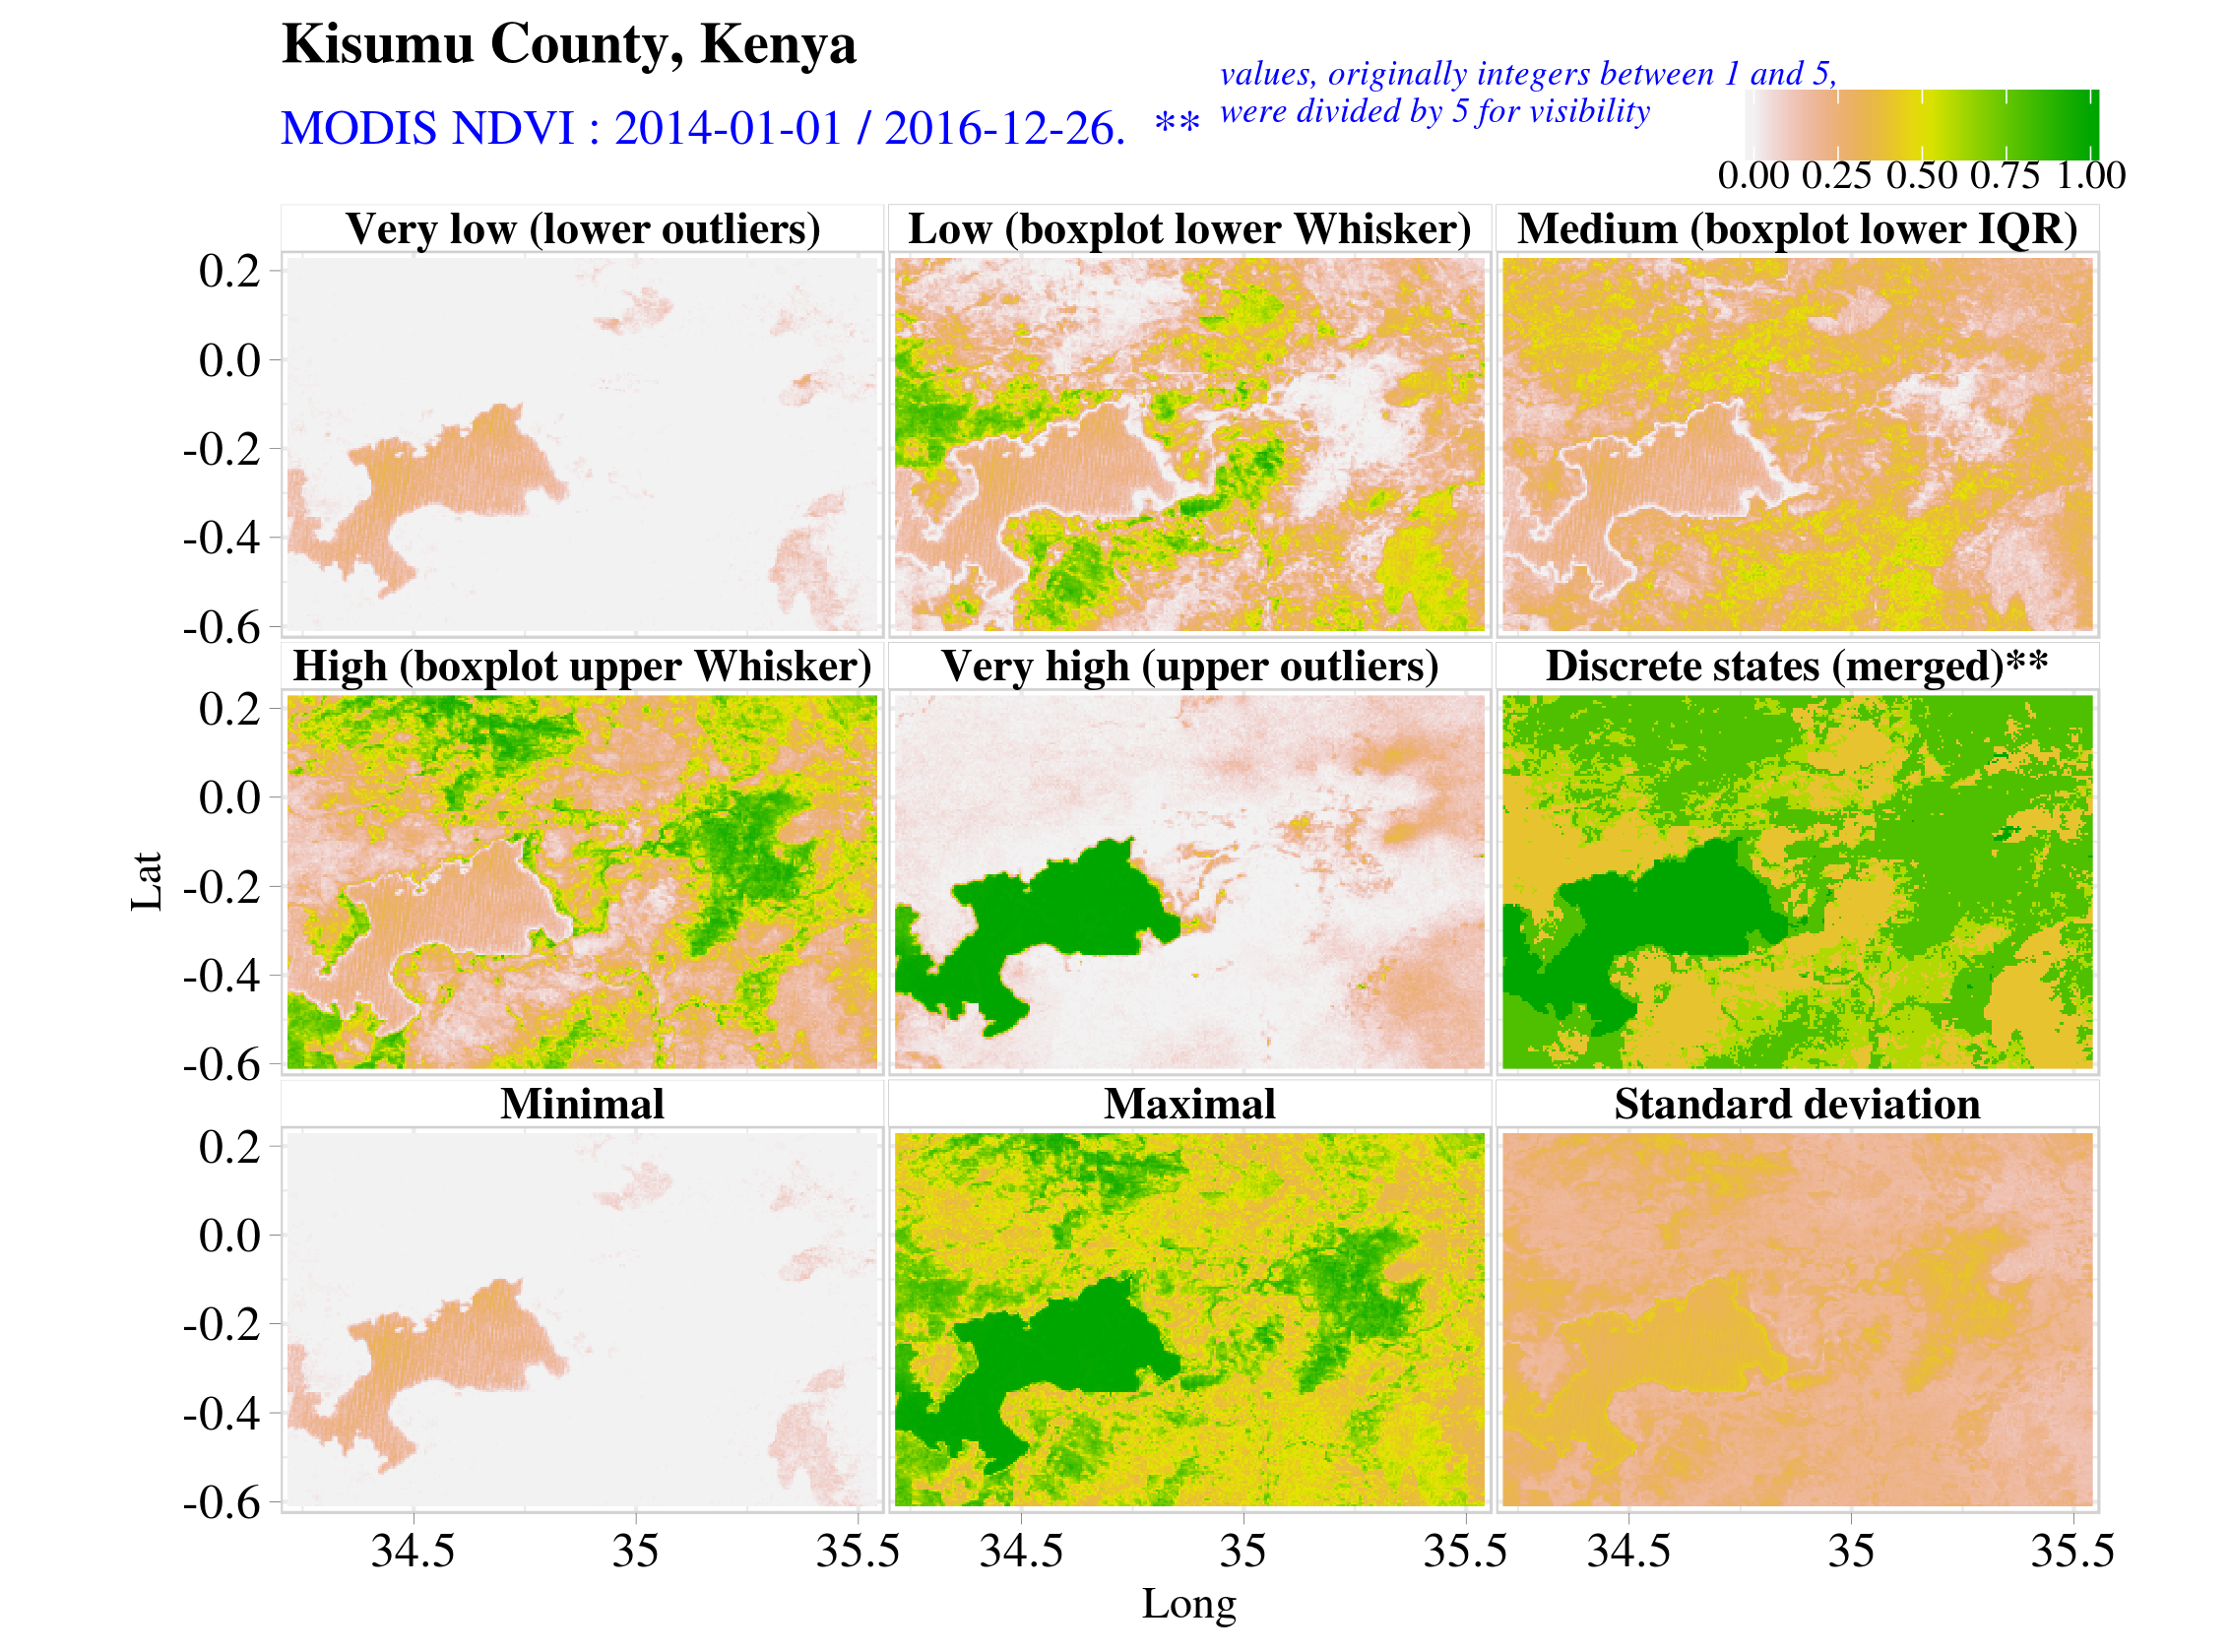
\includegraphics[width=1\linewidth]{figures/Mapping_FBFS_water_probability} \caption{Probability of water by ranges in Kisumu county, Kenya.}\label{fig:fig8}
\end{figure}

\begin{figure}
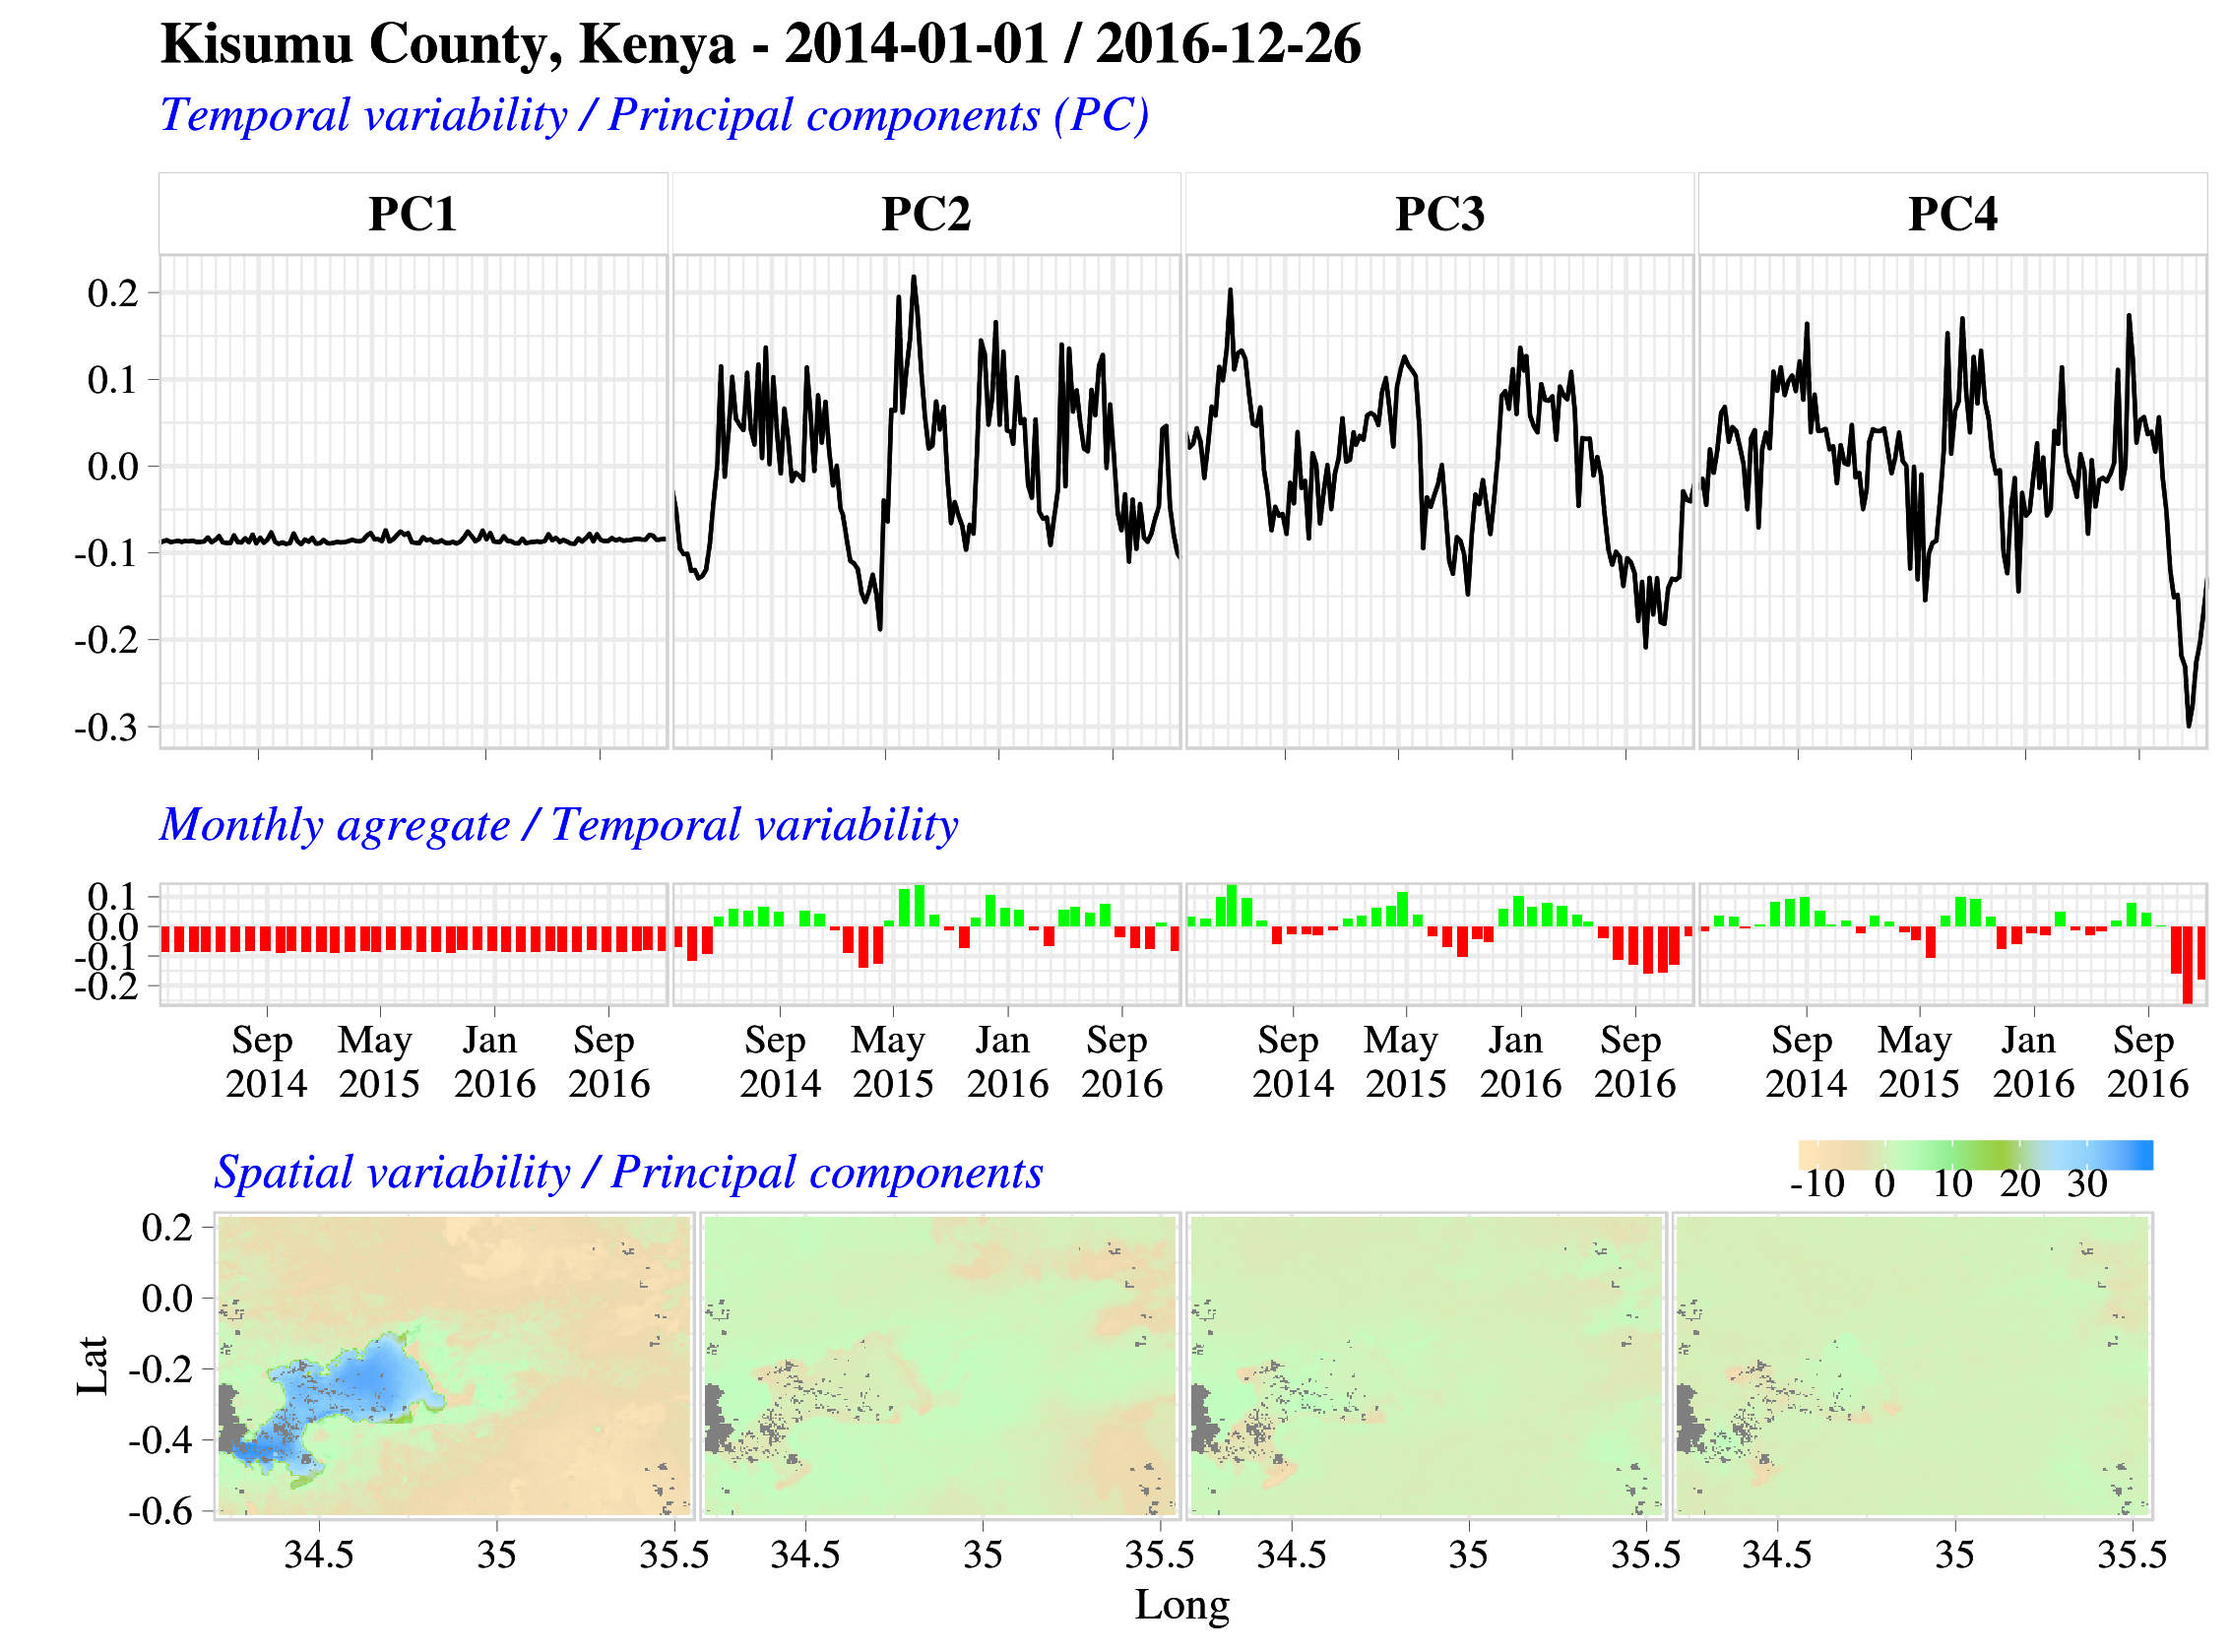
\includegraphics[width=1\linewidth]{figures/Mapping_FBFS_NDVI_PCA_plot_Kisumu} \caption{Dominants spatial and temporal characteristics of vegetation in Kisumu county, Kenya.}\label{fig:fig9}
\end{figure}

\begin{figure}
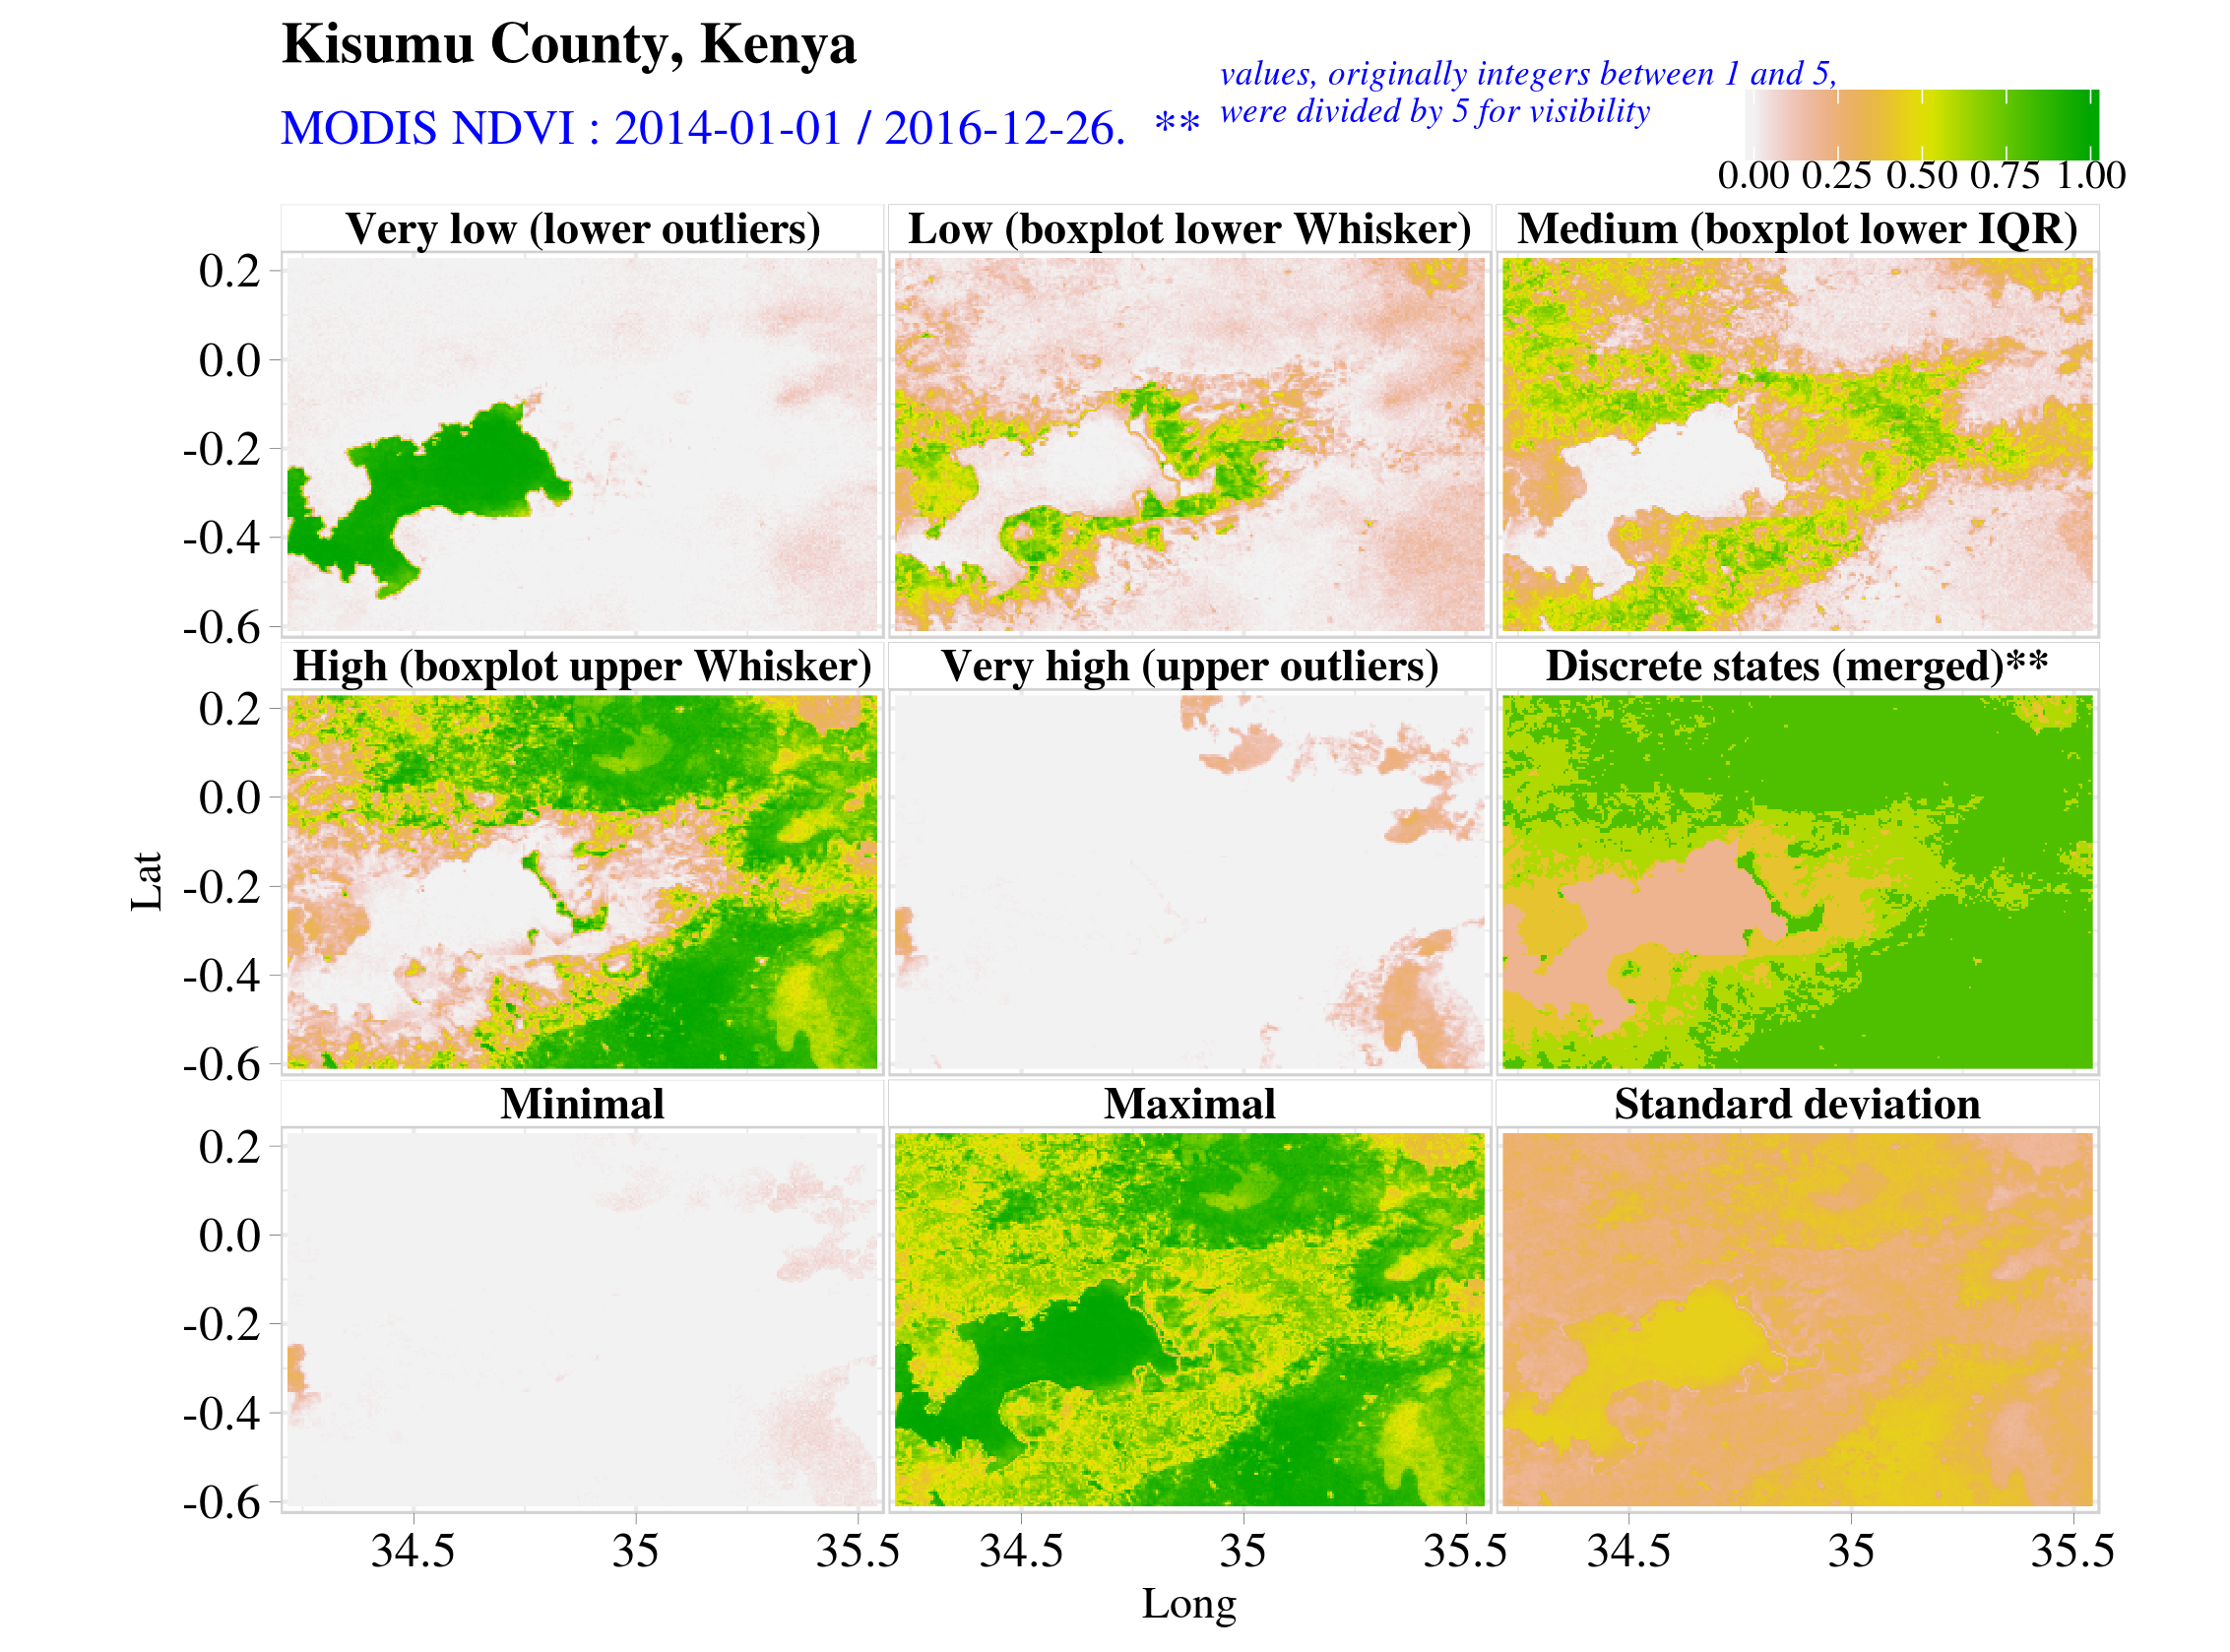
\includegraphics[width=1\linewidth]{figures/Mapping_FBFS_vegetation_probability} \caption{Probability of vegetation by ranges in Kisumu county, Kenya.}\label{fig:fig10}
\end{figure}

\hypertarget{II4}{%
\subsection{Prior spatial distribution of the spatial data node states}\label{II4}}

\begin{figure}
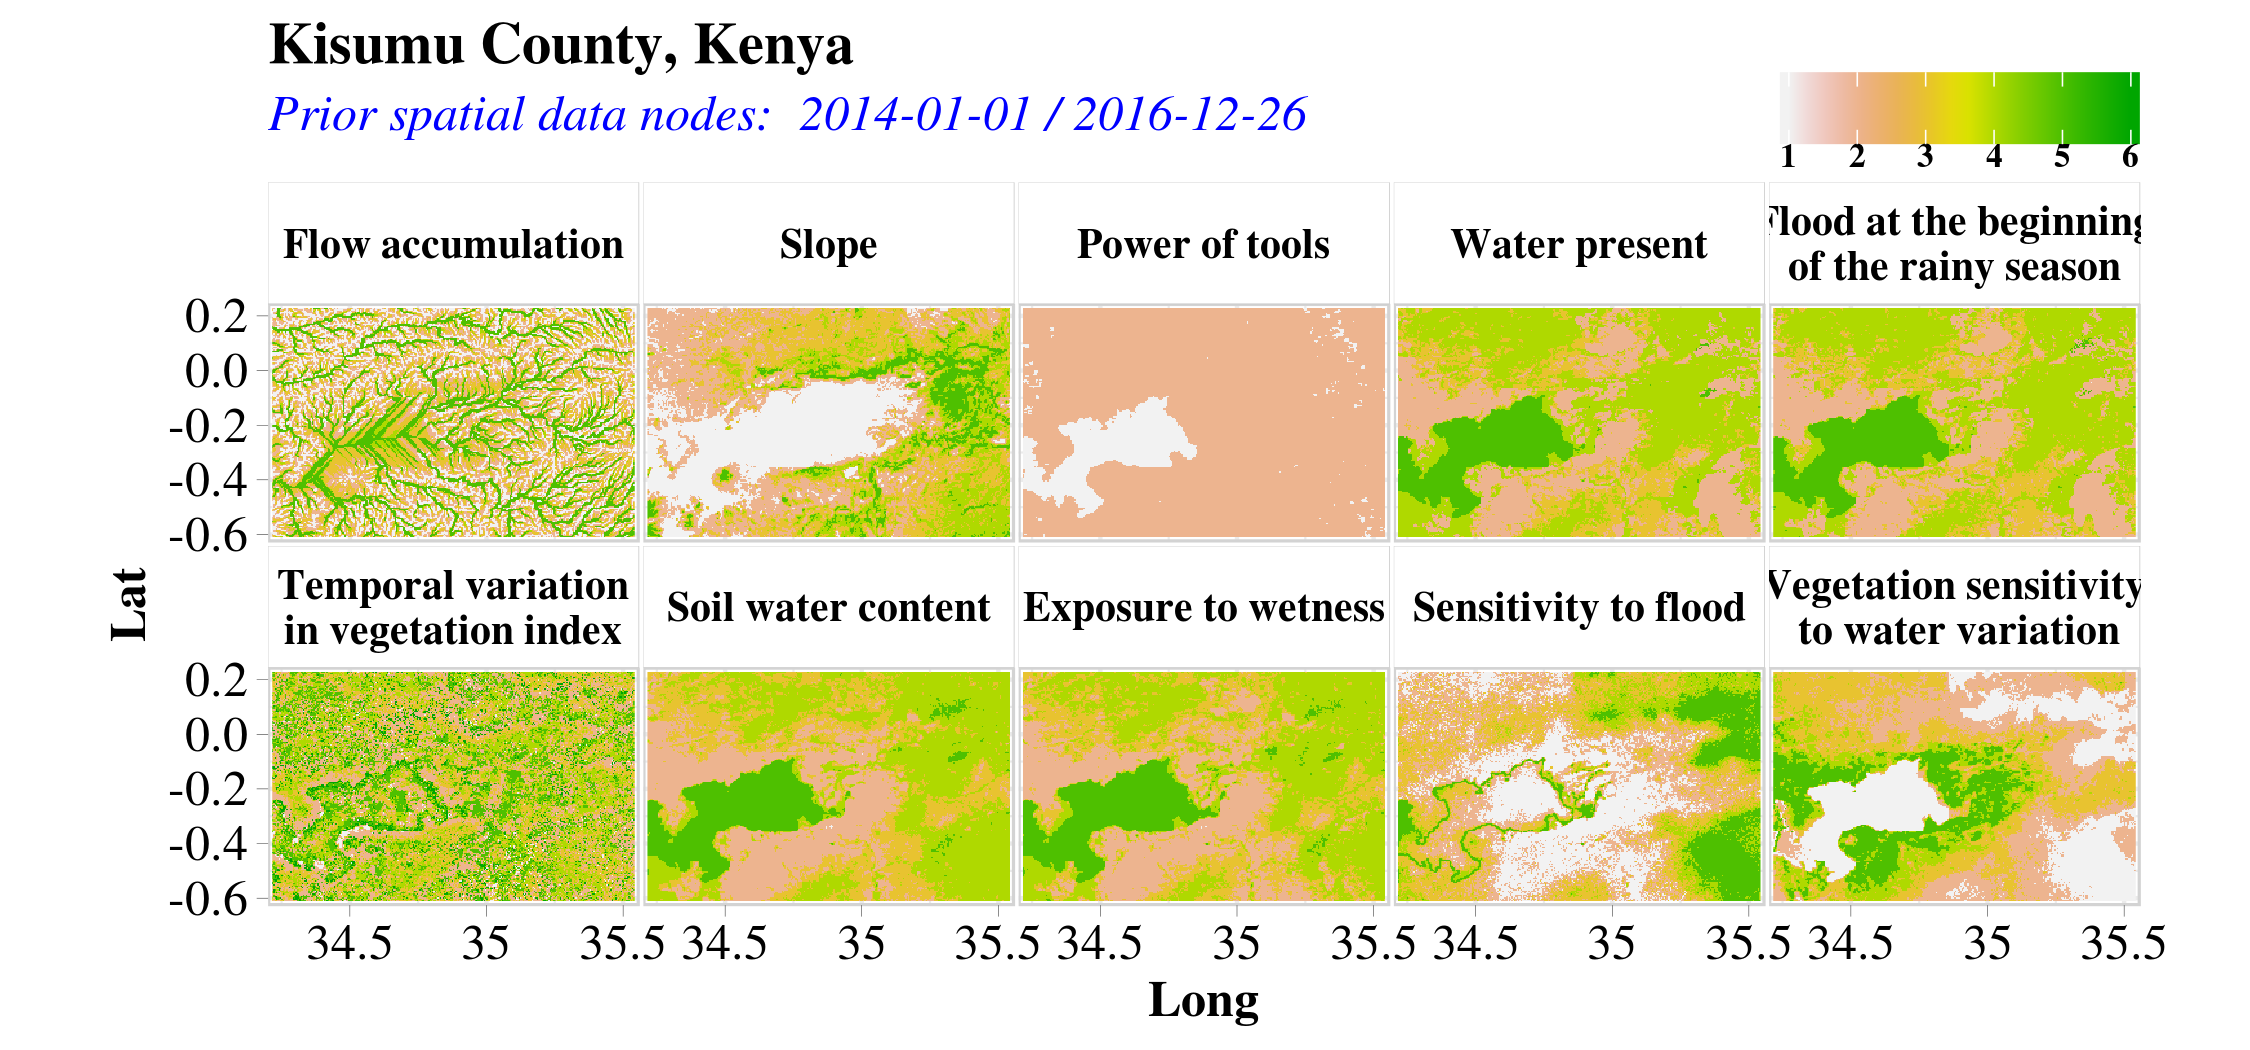
\includegraphics[width=1\linewidth]{figures/Mapping_FBFS_prior_maps} \caption{Prior spatial data used to feed the BNs for mapping FBFS in Kisumu county, Kenya.}\label{fig:fig11}
\end{figure}

\hypertarget{II5}{%
\subsection{Posterior spatial distribution of the spatial data node states}\label{II5}}

\begin{figure}
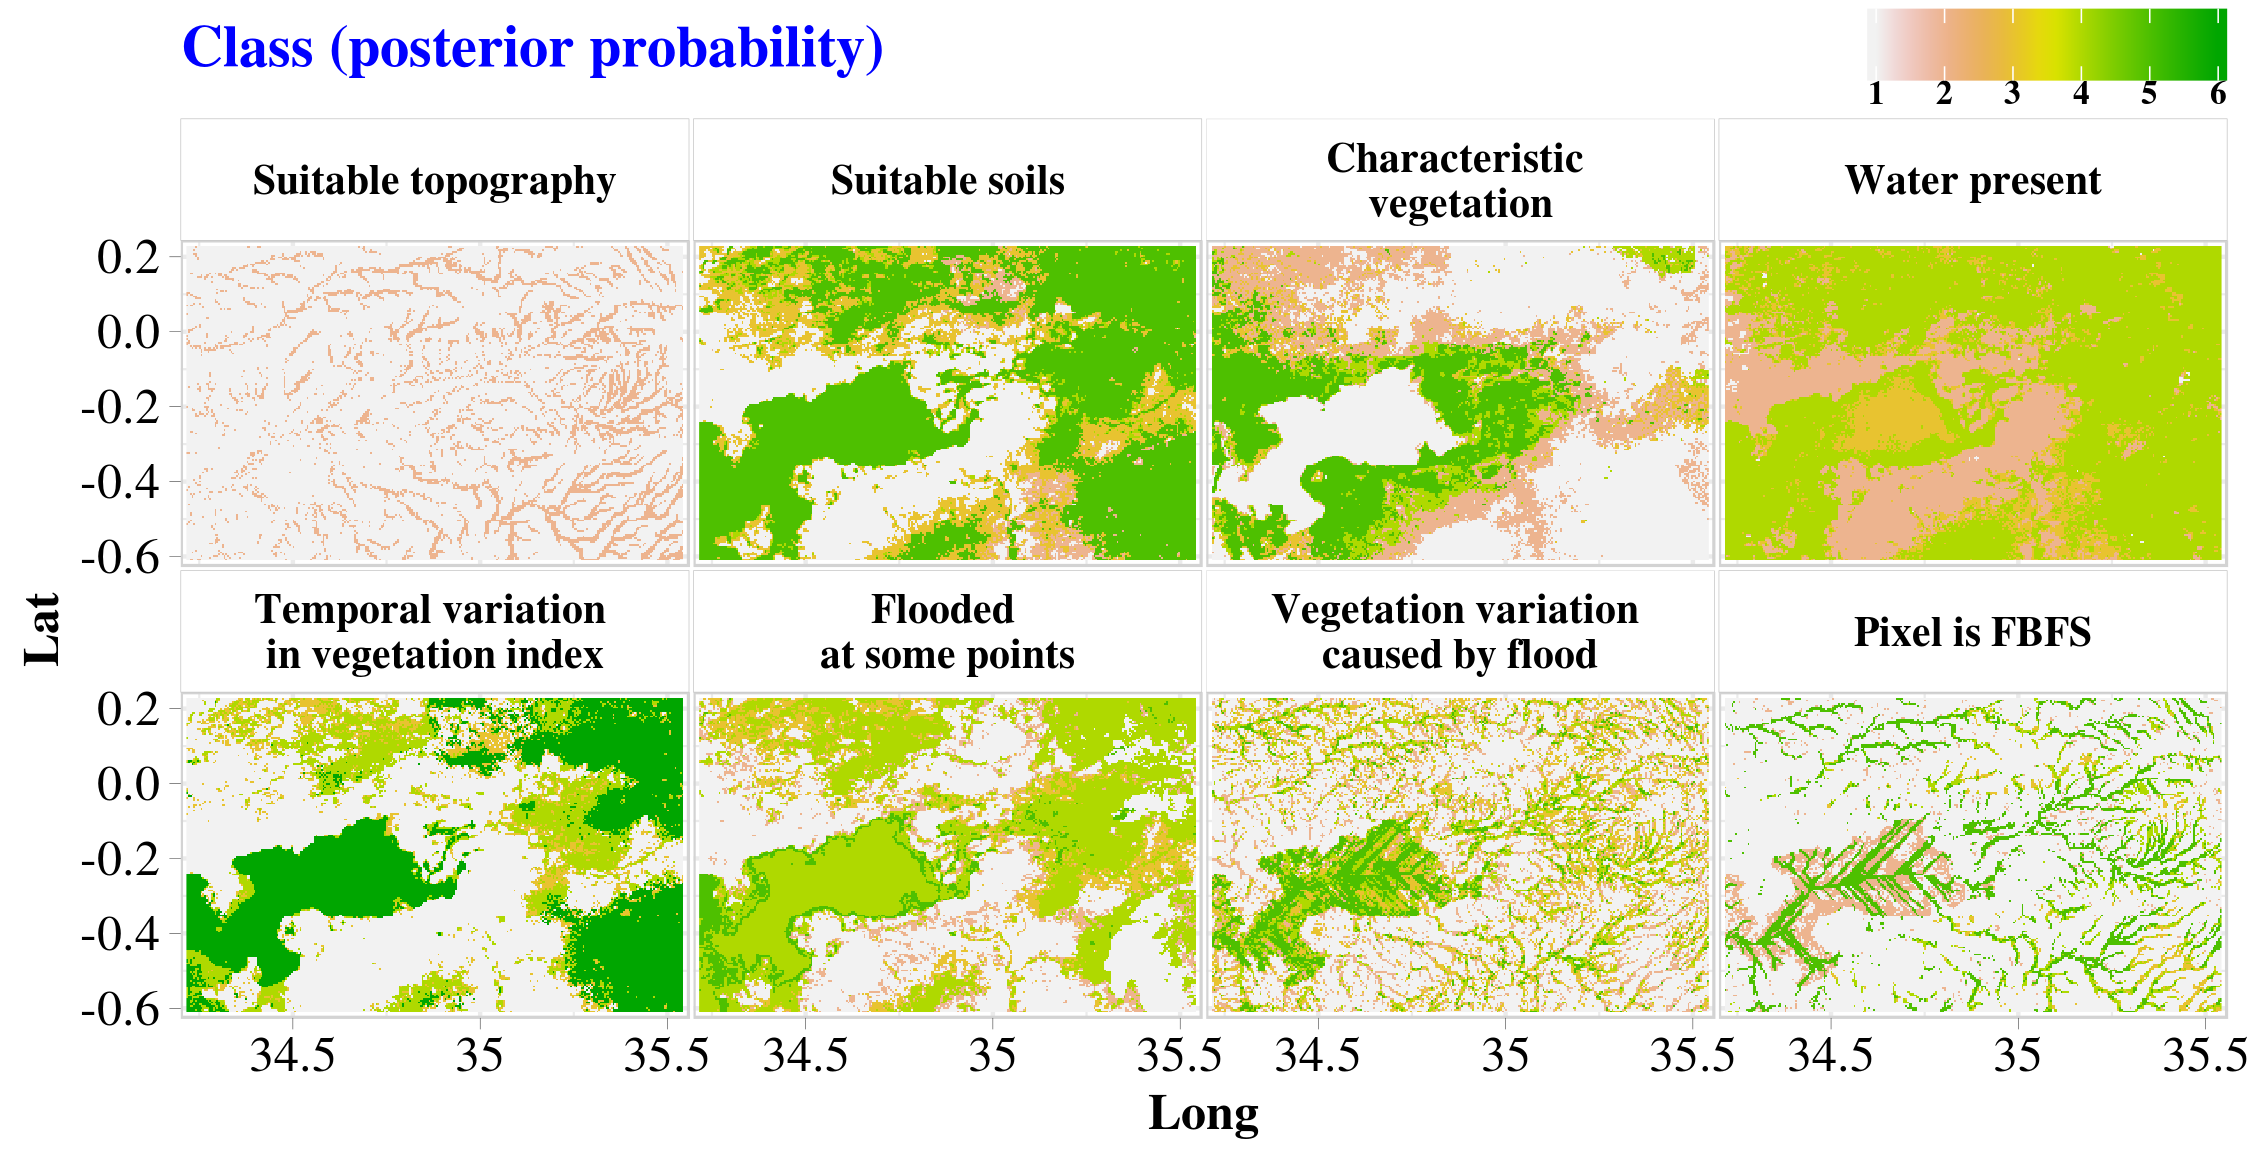
\includegraphics[width=1\linewidth]{figures/Mapping_FBFS_posterior_maps} \caption{Posterior FBFS maps and other important FBFS metrics in Kisumu county, Kenya.}\label{fig:fig12}
\end{figure}

\begin{figure}
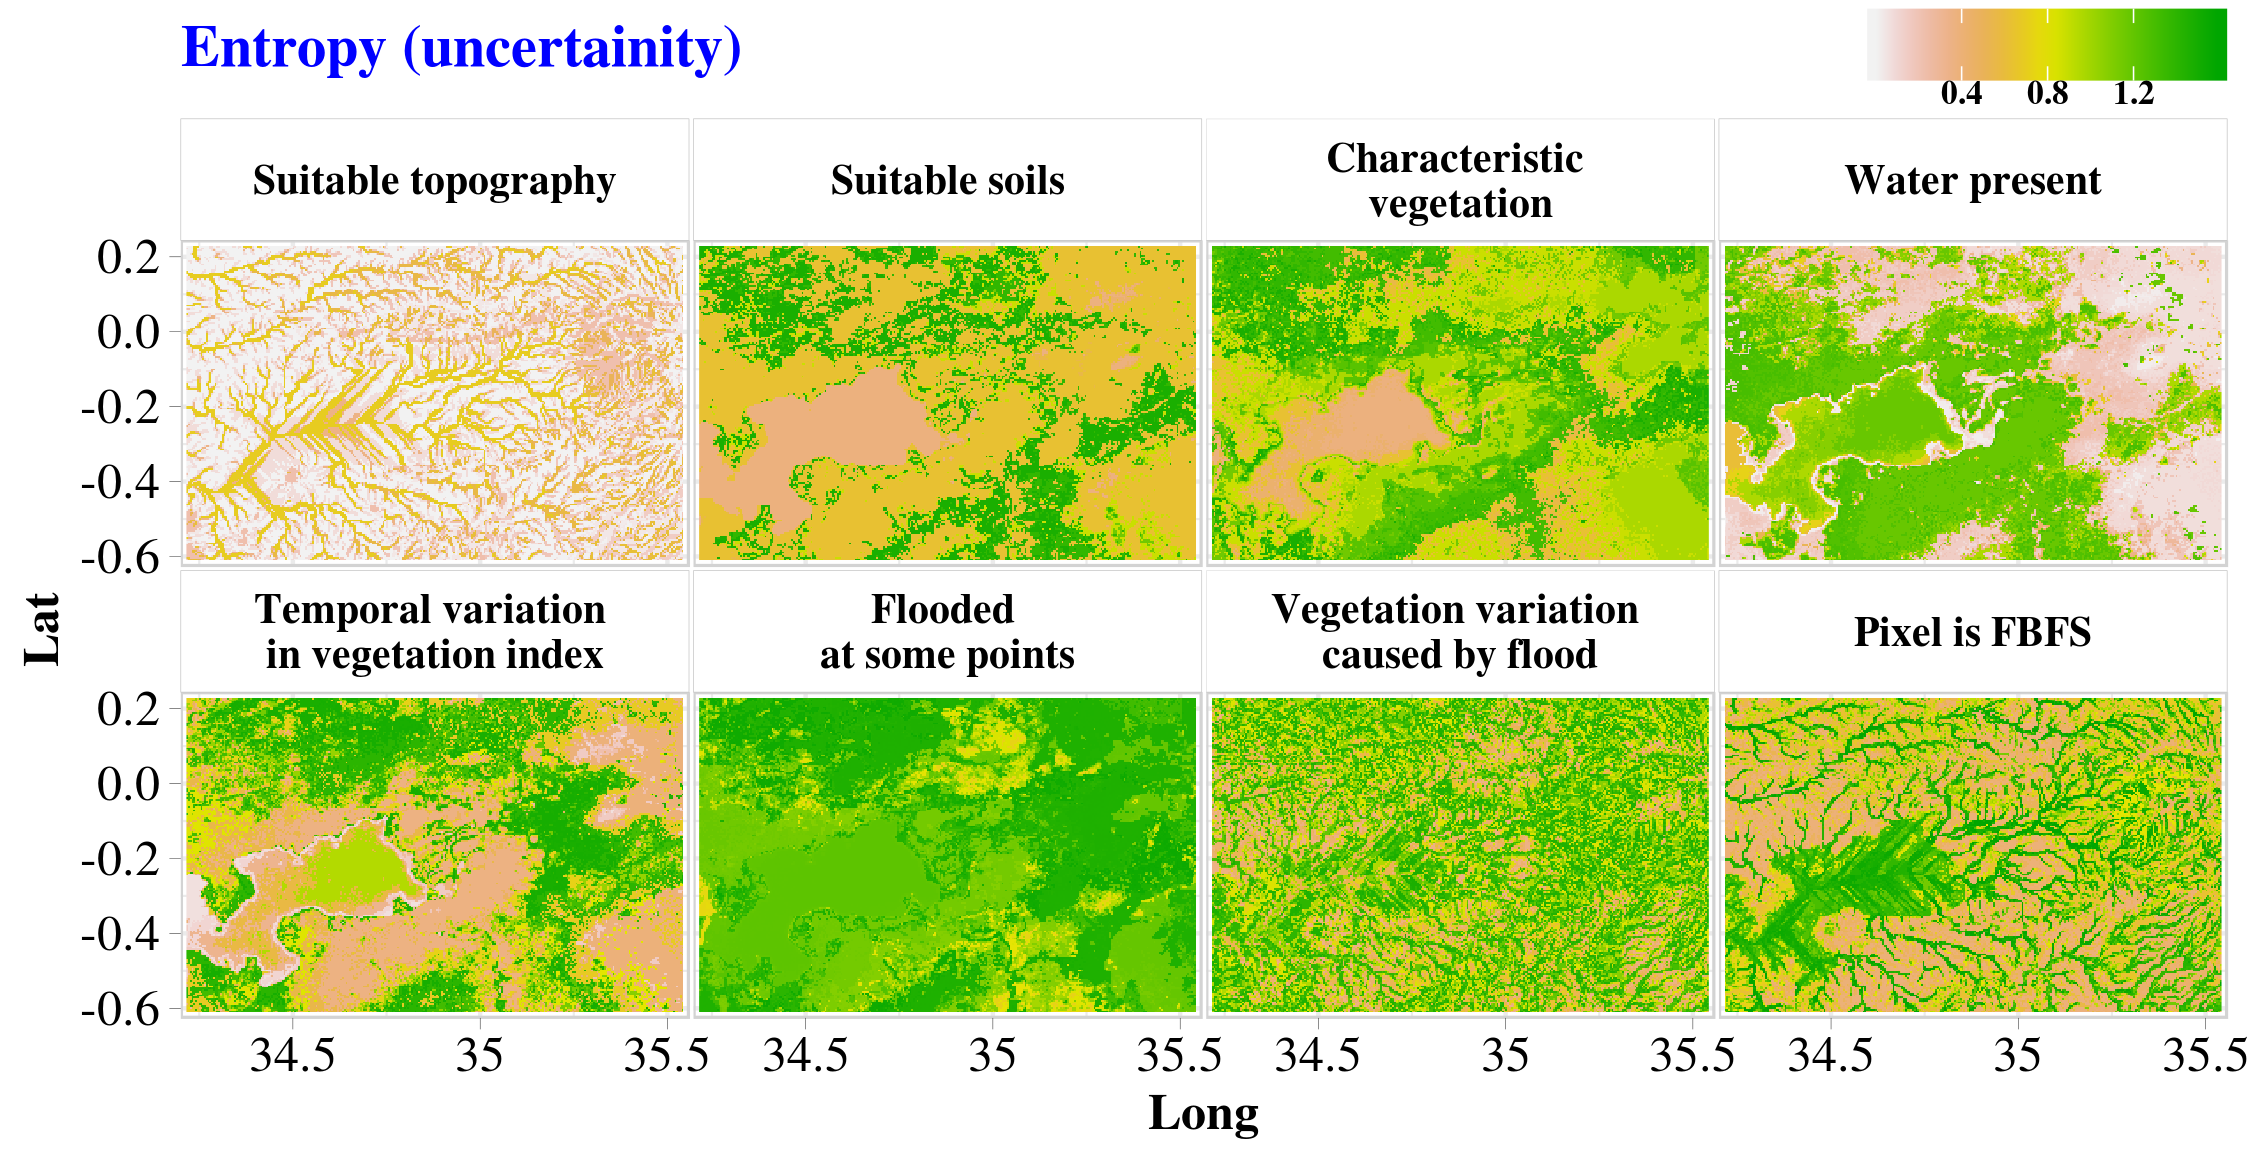
\includegraphics[width=1\linewidth]{figures/Mapping_FBFS_uncertainity_maps} \caption{Spatially explicit uncertainity maps derived as part of FBFS mapping in Kisumu county, Kenya.}\label{fig:fig13}
\end{figure}

\hypertarget{references}{%
\section*{References}\label{references}}
\addcontentsline{toc}{section}{References}

\hypertarget{refs}{}
\leavevmode\hypertarget{ref-Puertas_et_al_2011}{}%
1. Puertas, D. G.-L., Steenbergen, F. van, Haile, A. M., Kool, M. \& Embaye, T.-a. G. \emph{Flood based farming systems in Africa}. 52 (2011).

\leavevmode\hypertarget{ref-VanSteenbergen_et_al_2010}{}%
2. Steenbergen, F. van, Lawrence, P., Mehari, A., Salman, M. \& Faurès, J.-M. \emph{Guidelines on spate irrigation}. 249 (FAO, 2010).

\leavevmode\hypertarget{ref-Varisco_1983}{}%
3. Varisco, D. M. Sayl and ghayl: The ecology of water allocation in Yemen. \emph{Human Ecology} \textbf{11}, 365--383 (1983).

\leavevmode\hypertarget{ref-Xing_et_al_2014}{}%
4. Xing, L. \emph{et al.} China wetland extraction and classification using MODIS data. in \emph{2014 third international workshop on earth observation and remote sensing applications (eorsa)} 349--352 (IEEE, 2014).

\leavevmode\hypertarget{ref-FBLN_2018}{}%
5. FBLN. Flood-based Livelihood Network (FBLN) Foundation. (2018).

\leavevmode\hypertarget{ref-Haile_2010}{}%
6. Haile, A. M. \emph{A Tradition in Transition, Water Management Reforms and Indigenous Spate Irrigation Systems in Eritrea}. 212 (CRC Press, 2010).

\leavevmode\hypertarget{ref-Ghebreamlak_et_al_2018}{}%
7. Ghebreamlak, A. Z., Tanakamaru, H., Tada, A., Adam, B. M. \& Elamin, K. A. E. Satellite-based mapping of cultivated area in Gash Delta Spate Irrigation System, Sudan. \emph{Remote Sensing} \textbf{10}, 186 (2018).

\leavevmode\hypertarget{ref-Khalid_et_al_2016}{}%
8. Khalid, A. E. \emph{et al.} Performance Evaluation of Spate Irrigation Using Remote Sensing and DEM. in \emph{The 7th international conference on water resources and environment research (icwrer2016)} (ICWRER2016, 2016).

\leavevmode\hypertarget{ref-Theilen-Willige_et_al_2015}{}%
9. Theilen-Willige, B. \emph{et al.} Flash Floods in the Guelmim Area/Southwest Morocco--Use of Remote Sensing and GIS-Tools for the Detection of Flooding-Prone Areas. \textbf{5}, 203--221 (2015).

\leavevmode\hypertarget{ref-Boschetti_et_al_2014}{}%
10. Boschetti, M., Nutini, F., Manfron, G., Brivio, P. A. \& Nelson, A. Comparative analysis of normalised difference spectral indices derived from MODIS for detecting surface water in flooded rice cropping systems. \emph{PLoS ONE} \textbf{9}, (2014).

\leavevmode\hypertarget{ref-Wegmann_et_al_2016}{}%
11. Wegmann, M., Leutner, B. \& Dech, S. \emph{Remote Sensing and GIS for Ecologists: Using Open Source Software (Data in the Wild)}. 324 (Pelagic Publishing, 2016).

\leavevmode\hypertarget{ref-Konecny_2014}{}%
12. Konecny, G. \emph{Geoinformation: remote sensing, photogrammetry and geographic information systems}. 472 (CRC Press/Taylor \& Francis Group, 2014).

\leavevmode\hypertarget{ref-Bashari_et_al_2008}{}%
13. Bashari, H., Smith, C. \& Bosch, O. J. H. Developing decision support tools for rangeland management by combining state and transition models and Bayesian belief networks. \emph{Agricultural Systems} \textbf{99}, 23--34 (2008).

\leavevmode\hypertarget{ref-Hubbard_2014}{}%
14. Hubbard, D. W. \emph{How to Measure Anything: Finding the Value of Intangibles in Business}. 432 (John Wiley \& Sons, Inc., 2014).

\leavevmode\hypertarget{ref-Kuhnert_et_al_2010}{}%
15. Kuhnert, P. M., Martin, T. G. \& Griffiths, S. P. A guide to eliciting and using expert knowledge in Bayesian ecological models. \emph{Ecology Letters} \textbf{13}, 900--914 (2010).

\leavevmode\hypertarget{ref-Kuhnert_et_al_2005}{}%
16. Kuhnert, P. M., Martin, T. G., Mengersen, K. \& Possingham, H. P. Assessing the impacts of grazing levels on bird density in woodland habitat: A Bayesian approach using expert opinion. \emph{Environmetrics} \textbf{16}, 717--747 (2005).

\leavevmode\hypertarget{ref-Whitney_et_al_2018}{}%
17. Whitney, C., Shepherd, K. \& Luedeling, E. \emph{Decision analysis methods guide; Agricultural policy for nutrition}. 27 (2018). doi:\href{https://doi.org/10.5716/WP18001.PDF}{10.5716/WP18001.PDF}

\leavevmode\hypertarget{ref-Kuhnert_2011}{}%
18. Kuhnert, P. M. Four case studies in using expert opinion to inform priors. \emph{Environmetrics} \textbf{22}, 662--674 (2011).

\leavevmode\hypertarget{ref-Luedeling_et_al_2015}{}%
19. Luedeling, E. \emph{et al.} Fresh groundwater for Wajir - ex-ante assessment of uncertain benefits for multiple stakeholders in a water supply project in Northern Kenya. \emph{Frontiers in Environmental Science} \textbf{3}, (2015).

\leavevmode\hypertarget{ref-Whitney_et_al_2018a}{}%
20. Whitney, C. \emph{et al.} Probabilistic Decision Tools for Determining Impacts of Agricultural Development Policy on Household Nutrition. \emph{Earth's Future} \textbf{6}, 359--372 (2018).

\leavevmode\hypertarget{ref-Yet_et_al_2016}{}%
21. Yet, B. \emph{et al.} A Bayesian Network Framework for Project Cost, Benefit and Risk Analysis with an Agricultural Development Case Study. \emph{Expert Systems with Applications} \textbf{60}, 141--155 (2016).

\leavevmode\hypertarget{ref-Pourret_et_al_2008}{}%
22. Pourret, O., Naïm, P. \& Marcot, B. \emph{Bayesian Networks: A Practical Guide to Applications}. 446 (John Wiley \& Sons Ltd, 2008).

\leavevmode\hypertarget{ref-VanSteenbergen_et_al_2011}{}%
23. Steenbergen, F. van, MacAnderson, I. \& Mehari, A. \emph{Spate irrigation in the Horn of Africa: Status and potential.} 44 (2011).

\leavevmode\hypertarget{ref-Arge_et_al_2003}{}%
24. Arge, L. \emph{et al.} Efficient flow computation on massive grid terrain datasets. \emph{GeoInformatica} \textbf{7}, 283--313 (2003).

\leavevmode\hypertarget{ref-Gao_1996}{}%
25. Gao, B. C. NDWI - A normalized difference water index for remote sensing of vegetation liquid water from space. \emph{Remote Sensing of Environment} \textbf{58}, 257--266 (1996).

\leavevmode\hypertarget{ref-Hunt_and_Rock_1989}{}%
26. Hunt, E. R. \& Rock, B. N. Detection of changes in leaf water content using Near- and Middle-Infrared reflectances. \emph{Remote Sensing of Environment} \textbf{30}, 43--54 (1989).

\leavevmode\hypertarget{ref-Jenson_and_Domingue_1988}{}%
27. Jenson, S. K. \& Domingue, J. O. Extracting topographic structure from digital elevation data for geographic information system analysis. \emph{Photogrammetric Engineering and Remote Sensing} \textbf{54}, 1593--1600 (1988).

\leavevmode\hypertarget{ref-Ji_et_al_2009}{}%
28. Ji, L., Zhang, L. \& Wylie, B. Analysis of Dynamic Thresholds for the Normalized Difference Water Index. \textbf{75}, 1307--1317 (2009).

\leavevmode\hypertarget{ref-McFeeters_1996}{}%
29. McFeeters, S. K. The use of the Normalized Difference Water Index (NDWI) in the delineation of open water features. \emph{International Journal of Remote Sensing} \textbf{17}, 1425--1432 (1996).

\leavevmode\hypertarget{ref-Rouse_et_al_1973}{}%
30. Rouse, W., Haas, R. H. \& Deering, D. W. Monitoring vegetation systems in the Great Plains with ERTS, NASA SP-351. in \emph{Third earth resources technology satellite-1 symposium} 309--317 (NASA, 1973).

\leavevmode\hypertarget{ref-Roy_et_al_2014}{}%
31. Roy, D. \emph{et al.} Landsat-8: Science and product vision for terrestrial global change research. \emph{Remote Sensing of Environment} \textbf{145}, 154--172 (2014).

\leavevmode\hypertarget{ref-Tarboton_2003}{}%
32. Tarboton, D. Terrain analysis using digital elevation models in hydrology. in \emph{23rd esri international users conference} (2003).

\leavevmode\hypertarget{ref-Tucker_1979}{}%
33. Tucker, C. J. Red and Photographic Infrared Linear Combinations for Monitoring Vegetation. \emph{Remote Sensing of Environment} \textbf{08}, 127--150 (1979).

\leavevmode\hypertarget{ref-Yang_et_al_2006}{}%
34. Yang, X., Chapman, G. A., Young, G. A. \& Gray, J. M. Using Compound Topographic Index to delineate soil landscape facets from Digital Elevation Models for comprehensive coastal assessment. in \emph{MODSIM 2005 international congress on modelling and simulation. Modelling and simulation society of australia and new zealand} (2006).

\leavevmode\hypertarget{ref-RCoreTeam_2018}{}%
35. R Core Team. \emph{R: A language and environment for statistical computing.} (R Foundation for Statistical Computing, 2018).

\leavevmode\hypertarget{ref-KisumuCountyGovernment_2013}{}%
36. Kisumu County Government. \emph{Kisumu County First Integrated Development Plan 2013 - 2017.} (2013).

\leavevmode\hypertarget{ref-Farr_et_al_2000}{}%
37. Farr, T. G. \& Kobrick, M. Shuttle radar topography mission produces a wealth of data. \emph{Eos} \textbf{81}, 583--585 (2000).

\leavevmode\hypertarget{ref-Farr_et_al_2007}{}%
38. Farr, T. G. \emph{et al.} The shuttle radar topography mission. \emph{Reviews of Geophysics} \textbf{45}, (2007).

\leavevmode\hypertarget{ref-Nikolakopoulos_et_al_2006}{}%
39. Nikolakopoulos, K. G., Kamaratakis, E. K. \& Chrysoulakis, N. SRTM vs ASTER elevation products. Comparison for two regions in Crete, Greece. \emph{International Journal of Remote Sensing} \textbf{27}, 4819--4838 (2006).

\leavevmode\hypertarget{ref-Jarvis_et_al_2008}{}%
40. Jarvis, A., Reuter, H. I. I., Nelson, A. \& Guevara, E. Hole-filled seamless SRTM data V4. (2008).

\leavevmode\hypertarget{ref-Falorni_et_al_2005}{}%
41. Falorni, G., Teles, V., Vivoni, E. R., Bras, R. L. \& Amaratunga, K. S. Analysis and characterization of the vertical accuracy of digital elevation models from the Shuttle Radar Topography Mission. \emph{Journal of Geophysical Research: Earth Surface} \textbf{110}, (2005).

\leavevmode\hypertarget{ref-King_et_al_1995}{}%
42. King, M. D., Herring, D. D. \& Diner, D. J. The earth observing system (EOS): A space-based program for assessing mankind's impact on the global environment. \emph{Opt. Photon. News} \textbf{6}, 34--39 (1995).

\leavevmode\hypertarget{ref-Vermote_2015}{}%
43. Vermote, E. MOD09A1 MODIS/Terra Surface Reflectance 8-Day L3 Global 500m SIN Grid V006. (2015).

\leavevmode\hypertarget{ref-Pearl_2000}{}%
44. Pearl, J. \emph{Causality: Models, Reasoning and Inference}. 1--386 (Cambridge University Press, 2000). doi:\href{https://doi.org/citeulike-article-id:3888442}{citeulike-article-id:3888442}

\leavevmode\hypertarget{ref-GADM_2018}{}%
45. GADM. Database of Global Administrative Areas. (2018).

\leavevmode\hypertarget{ref-Hijmans_2019}{}%
46. Hijmans, R. J. raster: Geographic Data Analysis and Modeling. (2019).

\leavevmode\hypertarget{ref-Mattiuzzi_and_Detsch_2018}{}%
47. Mattiuzzi, M. \& Detsch, F. MODIS: Acquisition and Processing of MODIS Products. (2018).

\leavevmode\hypertarget{ref-Busetto_and_ranghetti_2016}{}%
48. Busetto, L. \& Ranghetti, L. MODIStsp: An R package for automatic preprocessing of MODIS Land Products time series. \emph{Computers \& Geosciences} \textbf{97}, 40--48 (2016).

\leavevmode\hypertarget{ref-GDAL_OGRcontributors_2018}{}%
49. contributors, G. GDAL/OGR Geospatial Data Abstraction software Library. (2018).

\leavevmode\hypertarget{ref-Bivand_et_al_2013}{}%
50. Bivand, R. S., Pebesma, E. \& Gómez-Rubio, V. \emph{Applied Spatial Data Analysis with R: Second Edition}. 405 (Springer New York, 2013).

\leavevmode\hypertarget{ref-Pebesma_Bivand_2005}{}%
51. Pebesma, E. \& Bivand, R. S. S classes and methods for spatial data: the sp package. (2005).

\leavevmode\hypertarget{ref-Mardia_et_al_1979}{}%
52. Mardia, K. V., Kent, J. T. \& Bibby, J. M. \emph{Multivariate Analysis}. 521 (Academic Press., 1979).

\leavevmode\hypertarget{ref-Pearson_1901}{}%
53. Pearson, K. On lines and planes of closest fit to systems of points in space. \emph{Philosophical Magazine} \textbf{2}, 559--57 (1901).

\leavevmode\hypertarget{ref-Leutner_et_al_2019}{}%
54. Leutner, B., Horning, N. \& Schwalb-Willmann, J. RStoolbox: Tools for Remote Sensing Data Analysis. (2019).

\leavevmode\hypertarget{ref-Likert_1932}{}%
55. Likert, R. A technique for the measurement of attitudes. \emph{Archives of Psychology} \textbf{22}, 5--55 (1932).

\leavevmode\hypertarget{ref-Wickham_and_Stryjewski_2012}{}%
56. Wickham, H. \& Stryjewski, L. \emph{40 Years of Boxplots}. 1--17 (2012).

\leavevmode\hypertarget{ref-Hothorn_et_al_2006}{}%
57. Hothorn, T., Hornik, K. \& Zeileis, A. Unbiased recursive partitioning: A conditional inference framework. \emph{Journal of Computational and Graphical Statistics} \textbf{15}, 651--674 (2006).

\leavevmode\hypertarget{ref-Roy_et_al_2002}{}%
58. Roy, D. \emph{et al.} The MODIS Land product quality assessment approach. \emph{Remote Sensing of Environment} \textbf{83}, 62--76 (2002).

\leavevmode\hypertarget{ref-Tarboton_1997}{}%
59. Tarboton, D. A new method for the determination of flow directions and upslope areas in grid digital elevation models. \emph{Water Resources Research} \textbf{33}, 309--319 (1997).

\leavevmode\hypertarget{ref-OCallaghan_Mark_1984}{}%
60. O'Callaghan, J. F. \& Mark, D. M. The extraction of drainage networks from digital elevation data. \emph{Computer Vision, Graphics, \& Image Processing} \textbf{23}, 323--344 (1984).

\leavevmode\hypertarget{ref-Tarboton_et_al_1991}{}%
61. Tarboton, D., Bras, R. L. \& Rodriguez‐Iturbe, I. On the extraction of channel networks from digital elevation data. \emph{Hydrological Processes} \textbf{5}, 81--100 (1991).

\leavevmode\hypertarget{ref-Tesfa_et_al_2011}{}%
62. Tesfa, T. K. \emph{et al.} Extraction of hydrological proximity measures from DEMs using parallel processing. \emph{Environmental Modelling and Software} \textbf{26}, 1696--1709 (2011).

\leavevmode\hypertarget{ref-Wallis_et_al_2009}{}%
63. Wallis, C., Watson, D., Tarboton, D. \& Wallace, R. Parallel Flow-Direction and Contributing Area Calculation for Hydrology Analysis in Digital Elevation Models. in \emph{The 2009 international conference on parallel and distributed processing techniques and applications} (2009).

\leavevmode\hypertarget{ref-DeLeeuw_et_al_2012}{}%
64. De Leeuw, J. \emph{et al.} Benefits of Riverine Water Discharge into the Lorian Swamp, Kenya. \emph{Water} \textbf{4}, 1009--1024 (2012).

\leavevmode\hypertarget{ref-Yu_et_al_2010}{}%
65. Yu, H., Luedeling, E. \& Xu, J. Winter and spring warming result in delayed spring phenology on the Tibetan Plateau. \emph{Pnas} \textbf{107}, 22151--22156 (2010).

\leavevmode\hypertarget{ref-Yu_et_al_2012}{}%
66. Yu, H., Xu, J., Okuto, E. \& Luedeling, E. Seasonal Response of Grasslands to Climate Change on the Tibetan Plateau. \emph{PLoS ONE} \textbf{7}, (2012).

\leavevmode\hypertarget{ref-White_et_al_1997}{}%
67. White, M. A., Thornton, P. E. \& Running, S. W. A continental phenology model for monitoring vegetation responses to interannual climatic variability. \emph{Global Biogeochemical Cycles} \textbf{11}, 217--234 (1997).

\leavevmode\hypertarget{ref-Nychka_et_al_2018}{}%
68. Nychka, D., Furrer, R., Paige, J. \& Sain, S. fields: Tools for Spatial Data. (2018).


\end{document}
